% Settings
% Settings
\newcommand{\doctitle}{Un servizio di visualizzazione di trasporti pubblici urbani su mappe \\for a Master Thesis}
\newcommand{\doctype}{Master Thesis}
\newcommand{\thesisauthor}{Valerio Lanziani}
\newcommand{\matriculation}{419447}
\newcommand{\academicyear}{2011/2012}
\newcommand{\supervisor}{Luca Cabibbo}
\newcommand{\cosupervisor}{asdasd}
\newcommand{\degree}{asdasd}
\newcommand{\university}{Università degli studi Roma 3}
\newcommand{\department}{Dipartimento di Ingegneria Informatica}
\newcommand{\logo}{contents/images/uni_roma3_logo.png}
\newcommand{\logowidth}{0.5 \linewidth}
\newcommand{\code}[1]{\texttt{#1}}

% Style Settings

% - Document Class
%\documentclass[dvipdfm,12pt,letterpaper,twoside,openright,english]{book}
\documentclass[a4paper,12pt,oneside,italian]{book}
% - ToC Depth
\setcounter{tocdepth}{2}
% - ToA Style
\newcommand{\tableofacronymstyle}{longheaderborder}
% - References Style
\newcommand{\mybibstyle}{ieeetr}

% Packages
\usepackage{listings}
\usepackage[12pt]{extsizes}
\usepackage{amsmath}
\usepackage{amsfonts}
\usepackage[pdftex]{graphicx}
\usepackage{xfor}
\usepackage[T1]{fontenc}
\usepackage{ae,aecompl}
\usepackage[nonumberlist,acronym,toc]{glossaries} 
\usepackage{longtable}
\usepackage{multirow}
\usepackage{setspace}
\usepackage[hyphens]{url}
\usepackage[pdftex]{hyperref}
\usepackage{cite}
\usepackage{setspace}
\usepackage{float}
\usepackage{epigraph}
%\usepackage[latin1]{inputenc}
%\usepackage[applemac]{inputenc}
\usepackage[utf8x]{inputenc}
\usepackage[italian]{babel}
\usepackage[belowskip=-10pt,aboveskip=0pt]{caption}

% Pages layout
\usepackage[top=35mm, bottom=25mm, left=35mm, right=35mm]{geometry}

% Enable glossaries
% Uncomment if you want to display all the entries (and not just the referenced ones)
\glsaddall
%
\newglossaryentry{Abcdefz}{name=Abcdefz,description={An \emph{abcdefz} is a Lorem ipsum dolor sit amet, consectetur adipiscing elit. Curabitur pharetra venenatis odio, ac pellentesque nulla blandit at. Maecenas eget massa arcu. Duis tempor justo et sapien ornare pulvinar}}
\newglossaryentry{Acderds}{name=Acderds,description={An \emph{acderds} is a Lorem ipsum dolor sit amet, consectetur adipiscing elit. Curabitur pharetra venenatis odio, ac pellentesque nulla blandit at. Maecenas eget massa arcu. Duis tempor justo et sapien ornare pulvinar}}
\newglossaryentry{Bpoiwne}{name=Bpoiwne,description={A \emph{bpoiwne} is a Lorem ipsum dolor sit amet, consectetur adipiscing elit. Curabitur pharetra venenatis odio, ac pellentesque nulla blandit at. Maecenas eget massa arcu. Duis tempor justo et sapien ornare pulvinar}}
\newglossaryentry{Csdfdse}{name=Csdfdse,description={A \emph{csdfdse} is a Lorem ipsum dolor sit amet, consectetur adipiscing elit. Curabitur pharetra venenatis odio, ac pellentesque nulla blandit at. Maecenas eget massa arcu. Duis tempor justo et sapien ornare pulvinar}}
%
%
\newacronym{ABC}{ABC}{Lorem ipsum dolor}
\newacronym{DEF}{DEF}{Lorem ipsum dolor}
\newacronym{GHI}{GHI}{Lorem ipsum dolor}
\newacronym{LMN}{LMN}{Lorem ipsum dolor}
%

\makeglossaries

% Interline
\linespread{1.5}

% PDF properties
\hypersetup{
colorlinks=false,
linktocpage=true,
plainpages=false,
pdfborder=0 0 0,
bookmarksopen=true,
pdftitle=\doctitle,
pdfauthor=\thesisauthor
}

% Set initial pagenumbering to none
%\setcounter{page}{0}
\pagestyle{empty}

% Indented Paragraph ;) - Use it like \begin{indentparagraph}{3cm}{your-paragraph}\end{indentparagraph}
\newenvironment{indentparagraph}[1]{\begin{list}{}{\setlength{\leftmargin}{#1}}\item[]}{\end{list}}


% Begin Document
\begin{document}

% Frontpage
\thispagestyle{empty}
\begin{center}
    \vspace{8mm}
    {\includegraphics[width=\logowidth]{\logo}} \\
    \vspace{8mm}
    {\large \university} \\
    \vspace{8mm}
    {\large \department} \\
    {\large \degree} \\
    \vspace{8mm}
    {\large \doctype} \\
    \vspace{10mm}
    {\large\bf \doctitle} \\
    \vspace{8mm}
    {\large Author \\ {\bf{\thesisauthor}} \\ Matr. \matriculation }\\
    \vspace{14mm}

    \begin{tabular}{c  @{\hspace{2.5cm}} c}
    Supervisor & Co-Supervisor \\
    \bf{\supervisor} & \bf{\cosupervisor} \\
    \end{tabular} \\

    \vfill
    {\large Academic Year \\ \academicyear} \\
\end{center}
\newpage

\cleardoublepage

% Dedication
%\null\vspace{\stretch{1}}
\begin{flushright}
{\it{

bla bla bla bla bla bla bla bla bla \\
bla bla bla bla bla bla bla bla \\
bla bla bla bla bla bla \\
bla bla bla bla bla bla bla bla bla \\
bla bla bla bla bla bla \\
- \\
Bla bla bla bla bla bla bla bla \\

}}
\end{flushright}
\vspace{\stretch{2}}\null
\newpage

%\cleardoublepage

% Abstract
%\chapter*{Abstract}{%
Lorem ipsum dolor sit amet, consectetur adipiscing elit. Curabitur pharetra venenatis odio, ac pellentesque nulla blandit at. Maecenas eget massa arcu. Duis tempor justo et sapien ornare pulvinar. Nullam sollicitudin aliquet dui, in fermentum tortor ornare eu. Duis cursus vehicula semper. Donec condimentum felis ut dolor malesuada imperdiet. Nam ullamcorper, tortor vitae mattis cursus, magna nulla interdum diam, sit amet egestas mi turpis nec metus. Ut eu est vitae dolor facilisis viverra. Praesent id erat eu diam semper tincidunt. Curabitur condimentum sem in neque gravida pulvinar. Aliquam vitae neque quis neque vehicula suscipit. Duis at purus felis. Vestibulum id ante ipsum. \\

Donec sit amet dui a arcu condimentum accumsan. Aliquam magna velit, pretium vitae placerat vel, mattis ut sapien. Aliquam porttitor ipsum quis risus ultricies non lacinia lorem laoreet. Integer elementum sollicitudin pulvinar. Donec sed ullamcorper orci. Suspendisse pretium ante ligula, a dapibus leo. Phasellus feugiat mauris vel lacus faucibus non ultricies ipsum placerat. Curabitur pellentesque odio nec eros egestas non pellentesque metus aliquam. Sed enim enim, interdum consequat consectetur sed, faucibus eu quam. Curabitur arcu massa, lacinia eu varius a, tempor id lacus. Praesent ultrices porttitor ligula, vitae consequat erat elementum eu. Aliquam vitae egestas justo. In hac habitasse platea dictumst. Ut interdum accumsan odio, eu commodo nunc laoreet vitae. Praesent purus nibh, tincidunt at viverra ut, bibendum quis lorem. Morbi convallis augue quis velit rhoncus non tristique est commodo.

}
%\thispagestyle{empty}
%\cleardoublepage

% Acknowledgements
\chapter*{Ringraziamenti}{\vspace{3cm}





{\large {\itshape Ringrazio la mia famiglia, il mio punto di riferimento, e i miei amici, i quali hanno sempre creduto in me.}}
\vspace{3cm}



\subsubsection{} % (fold)
\label{ssub:}

% subsubsection  (end)
{\large {\itshape Un ringraziamento speciale va a mio fratello Luca, il quale mi ha sempre sostenuto e spronato a dare il meglio di me.}}}
\thispagestyle{empty}
\cleardoublepage

% Starts Roman page numbering
\newpage
\setcounter{page}{1}
\pagenumbering{Roman}
\pagestyle{headings}

% ToC, LoF, LoT
\renewcommand{\contentsname}{Tabella dei contenuti}
\tableofcontents
\listoffigures
%\listoftables
\cleardoublepage

% Start page numbering
\newpage
\setcounter{page}{1}
\pagenumbering{arabic}

\chapter*{Introduzione}
\chaptermark{Introduzione}
{%
In ogni grande città di oggi viene offerto un vasto e complesso servizio di rete trasporti pubblici, svolto a garantire un sistema alternativo di trasporto per i cittadini che non possono o non vogliono utilizzare le vetture. Il problema di questi servizi risiede nella loro enorme struttura, la quale certe volte rende il sistema inefficiente portando a lunghe attese dei mezzi di trasporto. Vi è bisogno dunque di un sistema che permetta al cittadino di poter conoscere in anticipo la disponibilità dei mezzi e la loro ubicazione, in modo da ottimizzare al più possibile il tempo a sua disposizione. Nell'era moderna il tempo ormai è la cosa più preziosa a disposizione, e dunque la fornitura di questo sistema assume un ruolo ancora più importante nell'insieme. A maggior ragione, il sistema di monitoraggio deve risultare il più efficiente ed intuitivo possibile, in modo tale che il cittadino possa ottenere ciò che desidera evitando perdite di tempo.

L'obiettivo di questa tesi è dunque la realizzazione di un servizio web attraverso un apparato client-server capace di estrarre i dati relativi ad un sistema di trasporti da una risorsa web esterna, come il sito dei trasporti pubblici di Roma, e visualizzarli all'utente in maniera più semplice e diretta, mostrando le informazioni relative al transito degli autobus su una mappa interattiva.

Il lavoro è stato svolto da un team di due persone, dove io mi sono concentrato sulla richiesta dei dati e la loro opportuna visualizzazione mentre il mio collega si è focalizzato sull'apparato di estrazione dei dati.\\

Nel capitolo \ref{chapter:introduzione_al_problema} si descrive il concetto del problema, passando poi ad un'analisi approfondita dell'ecosistema su cui è stata posta l'attenzione ed una descrizione generale delle soluzioni e delle tecniche adottate per la realizzazione del servizio oggetto di questa tesi.\\

Il capitolo \ref{chapter:architettura} definisce la struttura del servizio ed i suoi requisiti architetturali, descrivendo l'architettura server-client ed il concetto di applicazione web moderna. In questa sezione viene specificato il comportamento di una webApp tramite il sistema di richieste AJAX ed il passaggio di informazioni tra server e client attraverso il formato JSON. Il capitolo prosegue descrivendo le specifiche del pattern MVC e le direttive REST, indispensabile per la progettazione di una buona applicazione web.\\

Nel capitolo \ref{chapter:modellazione} viene definita la struttura del diagramma del modello di dominio relativo all'ecosistema studiato in questa tesi. Fornendo una descrizione dei casi d'uso e una descrizione delle classi concettuali introdotte, fornendo alcuni esempi. Vengono dunque specificate le relazioni tra le classi e gli attributi di cui sono composte.\\

Il capitolo \ref{cha:progettazione} introduce alla progettazione del diagramma delle classi di progetto, proseguendo quanto introdotto nel capitolo precedente e portando ogni aspetto sotto un punto di vista applicativo, definendo le classi che dovranno essere realizzate nel progetto specificando i loro attributi e metodi, inoltre vengono definite tutte le associazioni e le dipendenze necessarie a far sì che le classi possano interagire l'una con l'altra.\\
\newpage

Conclusa la fase di progettazione, nel capitolo \ref{cha:frameworks} si descrivono le scelte di sviluppo, fornendo inizialmente una breve introduzione al linguaggio utilizzato, per passare poi allo studio di tre framework largamente utilizzati per lo sviluppo di applicazioni web: Ember.js, Spine.js e Backbone.js. Per ognuno viene dunque fornita una descrizione dei suoi aspetti principali e dei moduli a disposizione, valutando i vantaggi e gli svantaggi che ogni framework offre. Dopo aver completato la descrizione dei tre framework si apre una sezione sulla valutazione e la scelta del framework che verrà utilizzato per lo sviluppo del software, ponendo le loro caratteristiche a confronto.\\

Nel capitolo \ref{cha:realizzazione} viene descritta la realizzazione e lo sviluppo del servizio, introducento inizialmente gli svantaggi del linguaggio JavaScript e come questi siano stati risolti, descrivendo brevemente il formato common.js e AMD. Proseguendo si passa alla descrizione della struttura interattiva tra client e server, con quale interfaccia il client richieda le risorse ed in che modo il server provveda a renderle disponibili. Viene dunque posta la concentrazione sugli aspetti principali di questa tesi, descrivendo la struttura delle varie componenti del servizio in base al rispetto del pattern MVC. Vengono descritti i moduli dei modelli di interesse, il modulo di routing, la tecnica con cui i dati vengono richiesti al server e salvati nel client e la struttura per la gestione e la visualizzazione dei dati: le Viste. Viene quindi definito il concetto di template ed esaminate due librerie di templating in modo da farne utilizzo all'interno dell'applicazione. Si conclude il capitolo con le scelte ed i metodi per la visualizzazione dei dati su mappa, la definizione di responsive design ed i suoi pregi.\\

Il capitolo \ref{cha:dimostrazioni} descrive gli esempi d'uso dell'applicazione, mostrando come il servizio appare all'utente ed come questo funzioni. Come ultimo esempio viene mostrato una dimostrazione del design responsive.

La tesi si chiude col capitolo \ref{cha:conclusioni}, in cui vengono descritti gli obiettivi raggiunti e possibili sviluppi futuri per questo servizio.}
\addcontentsline{toc}{chapter}{Introduction}

% Chapters
\chapter{Il problema}\label{chapter:introduzione_al_problema}
Il settore dei trasporti è in continua evoluzione legata all'introduzione di nuovi materiali meno inquinanti, a titoli di viaggio multifunzioni (bus+treno) e a nuove tecniche di localizzazione dei mezzi, che lo riporta di grande attualità.

L’enorme importanza sociale dell’argomento ci impone lo sviluppo di questo settore lasciato per molti anni in balia di se stesso, contribuendo così ad aumentare e portare al collasso il traffico delle nostre città mentre il cittadino è arrivato alla “esasperazione/disperazione”.
Un semplice lavoro stradale, quale una contenuta pavimentazione, la rottura di una strada, in alcuni casi la modifica dei flussi viari, provocano disagi assai maggiori in oggettiva dimensione dell'evento.

La questione principale è il mancato rispetto degli orari di partenza o di transito che sono per l'utenza motivi di insoddisfazione ed incertezza che accrescono il già difficile rapporto delle Aziende con la loro clientela oltre alla critica negativa espressa dai cittadini nei confronti dei servizi offerti/organizzati dall’apparato statale/enti autonomi. A questo va aggiunta un’immagine negativa dell’Italia verso paesi stranieri.

In altri termini, in carenza di uno strumento idoneo che permetta di comunicare con tempestività a conducenti, personale di controllo, utenti, le modificazioni intervenute o le correzioni dei servizi tutto il sistema rischia il collasso, così il mezzo di trasporto non trova la possibilità di auspicare un servizio migliore. E' noto come le comunicazioni via etere siano di breve tempo e assolutamente indispensabili proprio in tutti quei casi in cui occorra tempestività e sicurezza.

Gran parte delle aziende di trasporto che operano nelle maggiori città italiane si sono dotate di software vari di gestione centralizzata in grado di rilevare i tempi di percorrenza degli autobus con la possibilità di rendere noti ai cittadini i tempi di attesa in alcune fermate. Questo ha contribuito a risolvere almeno tre questioni: il coordinamento della rete; l'informazione all'utenza; l’acquisizione dei dati di servizio, ai fini di una migliore utilizzazione dei mezzi pubblici e della predisposizione di adeguati piani di trasporto.
Va riconosciuto che, limitare la propria struttura operativa ad un sistema di ricetrasmissione vocale tra centro e personale sul territorio significa limitare di molto le potenzialità e soprattutto, utilizzarla prevalentemente come contingente, ma non certo per risolvere problemi.
Il primo di essi, coordinamento della rete dei servizi, è la diretta conseguenza dell’adozione del sistema di rilevamento della posizione dei mezzi e della loro rappresentazione grafica per segnalare scostamenti o irregolarità.

L'informazione all'utenza è lo strumento ideale per ristabilire quel colloquio, tra coloro che sono in attesa alle fermate oppure a bordo dei mezzi e l'Azienda.

L'acquisizione dei dati ``storici" del servizio rappresenta la fonte preziosa a cui attingere al momento di programmare orari ed itinerari dei nuovi programmi di esercizio.

Poter mantenere sotto generale controllo l'intera rete dei servizi viene ad essere molto importante fornirsi di sistemi informatici adeguati ed è dunque essenziale che ciò accada.

L'elemento coerente a tutto ciò deve però essere la possibilità di conoscenza e di intervento in tempo reale; una rete di servizi sottoposta a continuo monitoraggio ed un centro operativo attivo nel coordinamento sono gli elementi tecnici indispensabili.
Se poi, insieme ai dati di posizionamento, il mezzo invia anche i dati relativi all’affollamento dei passeggeri, ai tempi intercorsi per lo spostamento da un punto all'altro del suo itinerario relativi allo stato di efficienza del mezzo, il centro è in grado non solo di verificare la regolarità dei transiti ma, più in generale, lo ``stato" del servizio.

Ci si trova di fronte, inoltre, ed è proprio questo il motivo ispiratore di questo elaborato, ad un'utenza che ``vuole" essere informata con sufficiente anticipo, elemento che può far discendere la propria opzione di trasporto: una linea rispetto ad un'altra tenendo conto del tempo di attesa o, in altri casi, decidere di posticipare l'inizio del trasferimento.

La precisione perciò è, in questi casi, indispensabile. Viviamo in un momento storico in cui poter decidere come impiegare il tempo è particolarmente importante perché da esso dipende la qualità della vita.

Solo un sistema che si basi su dati ``reali" acquisiti direttamente dalla posizione degli autobus sulle rispettive linee può garantirla.
In questo lavoro, viene messo in risalto il servizio che si vuole offrire al cittadino utente, a colui che, poiché in prima linea, soffre dei disservizi e dei ritardi perché, in particolar modo nelle grandi città affida alla funzionalità del servizio di trasporto lo svolgimento della propria giornata. Nella frenesia dei tempi moderni, in cui si è sempre di corsa e con i minuti contati, è particolarmente importante poter scegliere modo e tempo degli spostamenti quotidiani siano essi riferiti all’attività lavorativa, sociale, al tempo libero o al recupero psico-fisico. Quindi si è deciso di mettere a disposizione del cittadino un’applicazione web ad alta tecnologia  ma di uso semplice.  Con un dispositivo abilitato alla navigazione nel web ogni utente potrà visualizzare la localizzazione degli autobus di interesse sull’intero territorio urbano e potrà scegliere quale linea preferire in relazione alla localizzazione dell’autobus. Egli, visualizzando l’intero percorso di tutte le linee, sceglierà i punti di salita e discesa più opportuni. Questa visualizzazione completa della mappa cittadina sul web è di grande supporto a tutti i cittadini, in particolar modo, a coloro che non sono esperti degli spostamenti all’interno della aree cittadine. Offre, quindi, un valore aggiunto a qualsiasi Azienda del settore in termini di servizi resi.

E’ d’obbligo chiarire che, nel nostro paese, ogni Azienda adotta un software di gestione centralizzata diverso da un’altra perché diverse sono le esigenze, le strutture, e tante altre cose ancora da città a città. Le varie Aziende non hanno svolto un lavoro comune per arrivare agli stessi risultati in  termini di servizi offerti al cittadino quindi, in alcune città, è possibile visualizzare gli orari di attesa su qualche fermata delle principali linee urbane, in altre questo risultato è ancora lontano ma si è lavorato su feed-back tra i tempi di percorrenza e gli affollamenti delle linee, in altre si sono ottenute entrambe le soluzioni sopra dette, ed in altre ancora si è lontano da  qualsiasi risultato che possa ottimizzare tempi di percorrenza e servizi di informazioni ai cittadini.

In ogni caso molte aziende di trasporto si sono dotate di software di gestione centralizzata per offrire un servizio  di informazione agli utenti e lavorano assiduamente per migliorare l’organizzazione di detto servizio in un ottica di ottimizzazione costi-benefici ma i software di cui si sono dotate, anche se contengono molteplici indicazioni: percorsi della linea, orari teorici di transiti agli orari feriali e festivi, ore di punta, di calma e serali, rischiano di fallire gli obiettivi perché di difficile lettura ed interpretazione; ciò senza considerare che forniscono elementi ``teorici" spesso vanificati e concorrono ad introdurre ulteriori elementi di incertezza. Essi devono riguardare i tempi di percorrenza reali, il numero dei passeggeri, la movimentazione alle rispettive fermate - saliti e discesi -, la ciclicità della richiesta di servizio e, più in generale, tutto quanto concorre a determinare orari. In questi casi avere a disposizione dati aggiornati sulla realtà delle situazioni non sono irrazionali richieste, ma può risultare assai utile per dimostrare che a fronte di un indubbio aggiornamento corrispondono analoghi benefici collettivi.

Proprio per la molteplicità delle prestazioni che un sistema integrato di gestione, di ricezione, trasmissione, messaggi e informazioni può offrire deve essere realizzato con attenzione.

La velocità dei flussi viari è facilmente deducibile analizzando i tempi di percorrenza dei bus e non è inutile valutare come gli stessi dati, riferiti ovviamente ai soli tempi di scorrimento del traffico, possano essere inviati anche al gestore dello stesso mantenendo sotto controllo la situazione viaria cittadina. Sarà quindi possibile per la stessa entità utilizzarli e, se nel caso, disporre una diversa temporizzazione dei cicli semaforici dando la necessaria priorità, rispetto alle altre componenti del traffico, a favore del trasporto pubblico.
Analogamente gli stessi dati potrebbero essere utilizzati per informare la veicolazione sia essa pubblica che privata.
Quindi dare un servizio di informazione precisa all’utente, oggi, con i potenti mezzi che l’elettronica offre,  è possibile e, soprattutto, si può aggiungere che, il cittadino ha bisogno di sentirsi al centro dell’attenzione, di sentirsi importante, di sentirsi parte integrante delle decisioni.

Un settore di così articolata composizione e difficoltà, non consente di affrontare una gestione centralizzata di un servizio di trasporto, se ad esso non concorrono conoscenze approfondite che difficilmente sono presenti in una singola entità.
Questo lavoro è stato pensato e creato mettendo il cittadino utente al centro dell’interesse. Quello che si raggiunge come scopo finale è la visualizzazione su mappa degli autobus di linea  che ogni utente potrà visualizzare ovunque si trovi utilizzando un dispositivo capace di navigare in rete (smart-phone, tablet, …)

\section{Obiettivo della tesi} % (fold)
\label{sec:section_name}

Come è stato appena introdotto, l'obiettivo di questa tesi è realizzare dunque un'applicazione web che permetta all'utenza di una grande città la consultazione di un servizio di trasporti pubblici, nel particolare la rete autobus urbana.
Per fare ciò vi è bisogno di progettare un servizio web che possa gestire gli accessi dell'utenza ed elaborare le informazioni che vengono richieste, per poi poter visualizzare i risultati di interesse all'utente.

E' stato preso come riferimento quindi il sistema dei trasporti pubblici romani ma, non potendo attingere a dati primitivi come, ad esempio, le coordinate GPS degli autobus in circolazione od una struttura chiara dell'intera ramificazione delle linee di roma, si è scelto di adottare un sistema di estrazione dei dati direttamente dal sito web che monitora la suddetta rete.
Altro problema già introdotto nella parte iniziale di questo capitolo risiede nella poca chiarezza della visualizzazione dei dati di interesse all'utente. Attualmente il sito web adibito al monitoraggio delle linee autobus gestisce  un basilare sistema di visualizzazione testuale, offrendo all'utente solamente dei tempi di attesa sui prossimi autobus in arrivo in ogni fermata, proprio come accade quando si attende un autobus in una fermata.
Disponendo di un servizio avanzato quale internet perché non fornire invece una visione più globale dell'intera rete dei trasporti? Sarebbe possibile ad esempio poter mostrare all'utente {\itshape tutti} gli autobus in circolazione su una direzione, visualizzando dove essi si trovano in ogni momento.
Su questo principio si basa il fulcro di questo servizio, e al fine di poter realizzare un sistema efficiente, vi è quindi bisogno della risoluzione di due problemi principali:

\begin{enumerate}
    \item estrarre i dati necessari dal sistema dei trasporti pubblici romani
    \item offrire una visualizzazione opportuna dei dati ricavati
\end{enumerate}

Per far fronte a queste problematiche viene dunque progettata una struttura server-client in cui il lato client sarà adibito alla richiesta dei dati di interesse e alla loro corretta visualizzazione, mentre il lato server si occuperà di servire le richieste del client ricavando i dati dal sistema web dei trasporti pubblici romani.

Questi aspetti sono stati realizzati attraverso una collaborazione tra due laureandi, lavorando comunemente per la risoluzione delle problematiche di estrazione e di visualizzazione.

Questo elaborato si focalizza sulla gestione lato client dei dati di interesse, descrivendo i metodi di richiesta e di organizzazione dei dati, come essi vengano visualizzati sulla mappa e la struttura dell'interfaccia web.

% section section_name (end)

\newpage


\chapter{Architettura del servizio}\label{chapter:architettura}
In questo capitolo viene introdotta una panoramica sulla struttuazione dell’architettura del servizio affinché possano essere soddisfatte le esigenze illustrate nel capitolo precedente.

Problematiche di questo tipo vengono risolte tramite lo sviluppo di un’applicazione web, o webApp cioè un'applicazione accessibile via web per mezzo di un network (es. una Intranet o la Rete Internet). Trattasi di un modello applicativo di elevata comodità, in quanto permette ad ogni utente di effettuare una consultazione interattiva delle informazioni di cui necessita.

Una webApp è strutturata su tre livelli: il primo livello è associabile al terminale di fruizione, il web browser; il secondo livello è costituito dal motore applicativo (core applicativo)  formato da codice sorgente in un qualche linguaggio di sviluppo dinamico lato-server (in questo caso Java); il terzo livello è riconducibile alla conservazione ed estrapolazione dei dati di interesse, cosicché possano essere riutilizzati in qualsiasi momento.

Una volta noto il funzionamento delle applicazioni web, per lo sviluppo di questo servizio si è scelto di utilizzare, come di consuetudine tra gli sviluppatori web, lo schema architetturale MVC.

Infine le risorse vengono definite e indirizzate tramite il REpresentational State Transfer (REST) cioè un tipo di architettura software per i sistemi di ipertesto distribuiti


\section{La Struttura Server-Client} % (fold)
\label{sec:la_struttura_server_client}

% section la_struttura_server_client (end)

% section section_name (end)

Per una webApp è necessaria un’architettura Server-Client, formata cioè da due parti ben distinte che comunicano attraverso un linguaggio ad esse comune.

Per far si che l’applicazione sia semplice da utilizzare ed accessibile alla maggior parte dell’utenza, è necessario che il progetto relativo al lato Client sia ben strutturato affinché sia facile la ricerca delle informazioni da parte dell’utente. E gestisca in maniera efficiente la mole di dati inviati dal Server.

Il Client, per sua natura, non compie operazioni complesse ma si limita a richiedere i dati di cui necessita, al server, per fornirne la visualizzazione. 

Il Server è l’entità complessa che gestisce tutta la mole di dati che servono affinché l’applicazione funzioni. Esso ha il compito di: ricevere le richieste del client, prelevare i dati da un gestore esterno o da un’altra fonte, trattarli opportunamente secondo la richiesta ricevuta e restituirli nella forma richiesta.

Secondo quanto sopra, è facilmente intuibile come il server si trovi a gestire un’elevata mole di dati e lo deve fare riducendo al minimo i tempi di attesa. Sono necessarie, quindi, performance elevate.

\newpage


\section{Applicazioni web: one page application} % (fold)
\label{sec:applicazioni_web_one_page_application}

Per comprendere il sistema che è alla base di questa architettura, si forniscono degli esempi. Essi partono da interazioni Cliet-Server di vecchio modello e arrivano a quelle di nuova generazione facendo notare la loro evoluzione. In un sito web tradizionale, l’esperienza dell’utente verrebbe trattata semplicemente facendo uso di una serie di reindirizzamenti come si può vedere dalla figura n.1 sotto riportata:

\begin{figure}[htbp]
\begin{center}
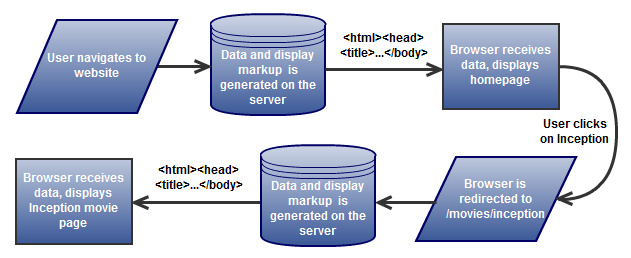
\includegraphics{contents/images/web_app_flow_2_1_}
\end{center}
\caption{}
\label{fig:flow_0}
\end{figure}

L’utente, tramite Client, accede al sito web; il server riceve e processa la richiesta ricevuta, genera i dati, li elabora se richiesto, e li invia con l’HTML necessario al client che, una volta ricevute le informazioni le elabora e consente la visualizzazione. A questo punto l’utente è in condizioni di navigare liberamente cercando quello di cui ha bisogno tenendo presente, però, che ad ogni singola richiesta corrisponde una nuova elaborazione, da parte del server, che dovrà generare nuovi dati, elaborati o non, per restituirli con l’HTML al client che verrà reindirizzato sulla pagina richiesta.
\newpage
Un’applicazione web di nuova generazione, ossia one page application, invece, previene qualsiasi reindirizzamento non necessario e permette la visualizzazione di diverse richieste in un’unica pagina, rendendo l’esperienza dell’utente molto più fluida e veloce come dalla figura n. 2 sotto riportata:

\begin{figure}[htbp]
\begin{center}
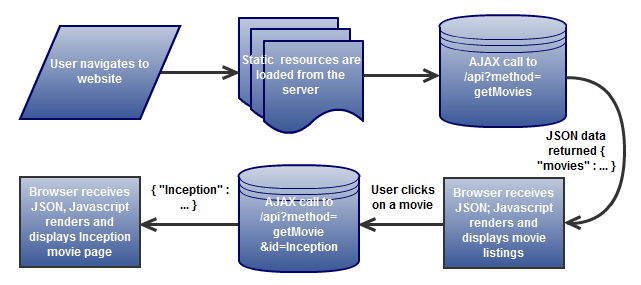
\includegraphics{contents/images/web_app_flow_3_1_}
\end{center}
\caption{}
\label{fig:flow_1}
\end{figure}

Qui, l’utente, tramite Client, accede al sito web ma, in questo caso, il server non elabora dati, né genera l’HTML, si limita a trasmette al browser tutte le risorse necessarie affinché possano essere elaborate per la creazione dei differenti aspetti della pagina. A questo punto inizia la navigazione dell’utente, il client invia le richieste al server tramite chiamate asincrone di tipo AJAX ed esso, processando quanto richiesto, restituirà solamente le informazioni che interesano. E’ compito del client occuparsi della visualizzazione corretta di quanto ricevuto utilizzando le risorse già in suo possesso.

Da questa breve trattazione si può notare come l’utilizzo di un’applicazione web di ultima generazione incrementi notevolmente la reattività del servizio. In queste webApp il carico di lavoro, non grava più esclusivamente sul server, ma viene ripartito tra i due lati. Questo permette al server di occuparsi della gestione dei dati e lascia tutti i compiti di presentazione al browser, che da semplice visualizzatore diventa, a tutti gli effetti, uno strumento attivo per la costruzione delle strutture di rappresentazione dei dati.

\newpage

\section{Il pattern MVC} % (fold)
\label{sec:il_pattern_mvc}

Una volta noto il funzionamento delle applicazioni web, per lo sviluppo di questo servizio si è scelto di utilizzare, come di consuetudine tra gli sviluppatori web, lo schema architetturale MVC.
MVC si basa sul concetto di applicazione basata su tre livelli: Model, View e Controller illustrato nella figura seguente:

\begin{figure}[htbp]
\begin{center}
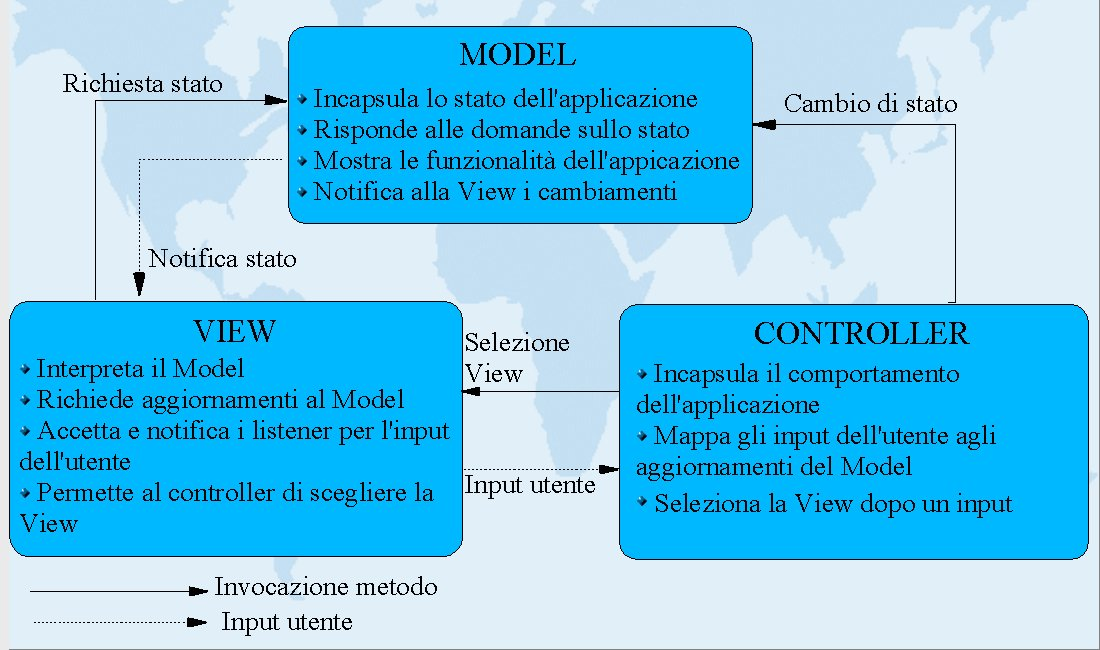
\includegraphics[width=10cm]{contents/images/mvc}
\end{center}
\caption{}
\label{fig:mvc}
\end{figure}



Il Model (modello) rappresenta lo strato che si occupa di fornire i metodi per l’accesso e la gestione dei dati primitivi (consultazione, modifica e salvataggio)  e la notifica alla View dei vari cambiamenti di stato.
Lo strato View (vista) si occupa solamente della metodologia di visualizzazione dei dati forniti dal modello per presentare, in maniera chiara e comprensibile, una rappresentazione dell’informazione.
Il Controller (controllore) ha il ruolo di ricevere i comandi dell’utente e formulare, di conseguenza, un’azione che risponda alle sue esigenze.
Quando l’utente formula una richiesta, il Controller si occupa di manipolare, attraverso dei comandi, i dati conservati nello strato Model. A seguito del cambiamento dei dati nel Model, lo strato View aggiornerà la loro rappresentazione in tempo reale. Concluso questo ciclo, potrà avere subito inizio una nuova richiesta. 
Utilizzando questo schema architetturale è possibile disaccoppiare e diminuire la coesione tra le varie componenti principali di un’applicazione che può essere esportata su qualsiasi piattaforma, al massimo dovrà essere rivisto il livello View per l’adattamento ai vari tipi di interfaccia grafica. 
L’esportazione di un’applicazione che non rispetta questo schema comporta il rifacimento dell’intera applicazione dovuta ad una elevata coesione della componente grafica verso tutte le altre impedendone l’uso. 

\section{Direttive REST} % (fold)
\label{sec:direttive_rest}

REpresentational State Transfer (REST) è un tipo di architettura software per i sistemi di ipertesto distribuiti come il World Wide Web e  si riferisce ad un insieme di principi di architetture di rete, i quali delineano come le risorse sono definite e indirizzate. I 5 principi fondamentali di questo tipo di architettura sono:
\begin{itemize}
    \item Il sistema deve essere necessariamente costituito da due parti ben distinte: Server-Client che interagiscono con interfacce comuni
    \item Il sistema deve essere stateless, ossia non si deve essere legati al fatto di dovere tenere aperte delle sessioni differenti da utente a utente. Quindi ogni richiesta fatta da ogni client può essere processata dal Server indipendentemente dalle richieste precedenti. Questo vincolo non impedisce però al Server di mantenere una cache di alcuni dati per migliorare le prestazioni e i tempi di risposta.
    \item Il sistema deve essere in grado di supportare una cache a diversi livelli. I browser commerciali sono in grado di eseguire il caching delle informazioni inviate dai vari server disponibili in Internet. Pertanto le risposte devono, implicitamente o esplicitamente, definire i livelli consentiti di cache al fine di supportare il client nell’ottimizzazione consistente delle performance.
    \item I sistemi devono essere accessibili in modo uniforme: ogni risorsa deve avere un indirizzo univoco globale e un punto valido di accesso. Ciò definisce un’interfaccia uniforme che permette un elevato grado di disaccoppiamento tra client e server.
    \item Il sistema deve essere stratificato. Un client internet normalmente non è in grado di determinare se è connesso direttamente con il server o se è connesso attraverso un agente intermedio.
    \item Questo è un vincolo facoltativo: i sistemi coinvolti devono essere in grado di estendere temporaneamente o di personalizzare le funzionalità al lato client attraverso il trasferimento di codice eseguibile. Alcuni esempi sono dati dal trasferimento di componenti eseguibili come le applet Java o di script sorgenti come JavaScript.
\end{itemize}

L’architettura REST permette oggi di avere servizi Web scalabili, efficienti e raggiungibili da chiunque ed ovunque. Seguendo questi principi di ha la possibilità di testare il funzionamento di un’applicazione per mezzo di un semplice browser commerciale. Ciò è particolarmente utile anche durante le fasi iniziali di implementazione dell’integrazione.

\newpage


\chapter{Modellazione}\label{chapter:modellazione}
In questo capitolo verrà trattata la fase di modellazione, che rappresenta la fase principale di ogni processo di sviluppo di un'applicazione.

Attraverso la modellazione è possibile definire un {\itshape modello di dominio}, il quale assume il compito di descrivere un ecosistema di entità del mondo reale che interagiscono tra loro, attraverso una rappresentazione grafica per mezzo di diagrammi.

Per poter apprendere i metodi di sviluppo di un modello di dominio vi è prima di tutto il bisogno di comprendere il concetto di Analisi Orientata agli Oggetti (OOA) e Progettazione Orientata agli Oggetti (OOP). Inoltre è di notevole aiuto conoscere i concetti base di UML, una notazione standard per la creazione di diagrammi.

\section{Analisi e Progettazione \\ Orientata agli Oggetti} % (fold)
\label{sec:analisi_orientata_agli_oggetti}

Prima ancora di definire il concetto di Analisi Orientata agli Oggetti vi è il bisogno di soffermarsi sul significato di analisi.
Come il termine stesso indica, l'analisi enfatizza un'investigazione del problema e dei requisiti in un universo di riferimento, anziché una soluzione. Nell'esempio di questo ambiente di studio, bisogna prima di tutto comprendere il funzionamento di un sistema di trasporti urbani e le sue proprietà.
Al contrario, la progettazione enfatizza una soluzione concettuale che soddisfa i requisiti, anziché la relavita implementazione. Infine il progetto può essere implementato, e l'implementazione (ovvero il codice) esprime il progetto realizzato vero e proprio.

Dunque nell'analisi orientata agli oggetti vi è un'enfasi sull'identificazione e la descrizione di oggetti, o di concetti, nel dominio del problema. Durante la progettazione orientata agli oggetti l'enfasi è sulla definizione di oggetti software e del modo in cui questi collaborano per soddisfare i requisiti.
% section analisi_orientata_agli_oggetti (end)

\section{UML (Unified Modeling Language)} % (fold)
\label{sec:uml_}

L'Unified Modeling Language, o UML, è un linguaggio di modellazione e specifica basato sul paradigma orientato agli oggetti. Esso rappresenta 
uno standard {\itshape de facto} per la notazione di diagrammi per disegnare o rappresentare figure relative al software, ed in particale relative al software OO.
UML consente di costruire modelli OO per rappresentare domini di diverso genere. Nel contesto dell'ingegneria software, viene utilizzato soprattutto per descrivere il dominio applicativo di un sistema software e/o il comportamento e la struttura del sistema stesso.
Il modello è strutturato secondo un insieme di viste che rappresentano diversi aspetti della cosa modellata, sia a scopo di analisi che di progetto, mantenendo la tracciabilità dei concetti impiegati nelle diverse viste. Oltre che per la modellazione dei sistemi software viene usato per descrivere domini di altri tipi, ad esempio sistemi hardware, sistemi di gestione o strutture organizzative in un'ecosistema specifico. 
% section uml_ (end)

\section{Il MDD della rete trasporti pubblici} % (fold)
\label{sec:il_MDD_della_rete_trasporti_pubblici}

Come si è già accennato in precedenza, una rete di trasporti pubblici di notevoli dimensioni comporta una ramificazione dei trasporti attraverso un'agglomerato di linee. L'azienda dei trasporti deve fornire un metodo di consultazione semplice e chiaro così da permettere ad un qualsiasi cittadino di comprendere come funzioni il sistema.

Viene ora descritto un possibile caso d'uso per la consultazione del servizio di trasporti:

\begin{enumerate}
   \item un {\bfseries utente} consulta un'elenco di {\bfseries linee} per scegliere quella d'interesse
   \item l'{\bfseries utente} sceglie una {\bfseries direzione} di preferenza appartenente alla linea selezionata
   \item dunque consulta l'elenco di {\bfseries fermate} del tracciato preso in esame
   \item l'{\bfseries utente} sceglie dunque la {\bfseries fermata} in base alla sua {\bfseries posizione}
   \item l'{\bfseries utente} consulta dunque gli {\bfseries autobus} in arrivo
\end{enumerate}

Dall'elenco dell'analisi dei nomi e delle locuzioni nominali è possibile generare un elenco delle classi concettuali candidate per il dominio. Dal momento che si tratta di un sistema di trasporti pubblici, si pone l'attenzione prima di tutto sulle categorie che enfatizzano oggetti fisici e le relazioni tra di essi.
Come già visto da alcuni esempi precedenti, si possono individuare alcune classi principali di rilievo:

\subsubsection{Linea} % (fold)
\label{ssub:linea}
In una rete di trasporti pubblici, una linea specifica una direzione (o molteplici direzioni) con il quale l'azienda dei trasporti desidera ricoprire un settore di città, potendo offrire ai cittadini che risiedono in quella zona un servizio di trasporto. Una linea è frequentemente rappresentata da un numero o un codice. 

Si faccia attenzione a non confondere una linea con una direzione: al contrario di quest'ultima, la linea non è strutturata su un ben preciso percorso e su una serie di snodi stradali, ma raffigura un ramo della rete dei trasporti che ricopre una porzione della città in cui l'azienda è situata.

L'azienda dei trasporti sarà dunque composta da numerose linee, che attraverso le loro ramificazione portano a ricoprire tutta la metropoli, garantendo un servizio equo per tutti i cittadini.

Attraverso le direzioni le linee tendono a ricongiungersi ad uno o più punti di snodo centrali, permettendo, a chi ha bisogno di percorrere lunghi tratti, la possibilità di cambiare linea e raggiungere dunque altri settori differenti di città.
% subsubsection linea (end)

\subsubsection{Direzione} % (fold)
\label{ssub:direzione}
Una direzione rappresenta un preciso percorso offerto da una linea, il percorso si snoda attraverso un tragitto specifico tra le strade della città.

Una direzione è specificata anche dal verso di percorrenza, dunque anche se una linea offre un solo percorso, tipicamente essa dispone di due direzioni che ne definiscono il tragitto di andata e di ritorno.

In ogni direzione vengono specificati dei punti di sosta, situati in punti di interesse o in zone particolarmente visitate da cittadini e turisti. In ogni punto di sosta risiede una fermata, o stazione, in cui è possibile richiedere ai mezzi pubblici la sosta per la  salita e la discesa dei passeggeri.

Nei punti di inizio e di fine di una direzione è collocata la fermata di capolinea. Due direzioni aventi lo stesso percorso ma con versi di percorrenza dfferenti hanno in comune le stesse fermate di capolinea, permettendo agli autobus che concludono una direzione di invertire rotta e procedere nella direzione inversa.

In una linea può però capitare che anche avendo solo due direzioni, queste due non condividino lo stesso percorso. In questi casi le due direzioni passano attraverso vie differenti o solo parzialmente differenti, ricongiungendosi infine nella stazione di capolinea.

Ogni direzione è rappresentata attraverso un nome o un codice, o in alcuni casi, dalla combinazione dei due. Il nome tipicamente si riferisce al verso di percorrenza del tragitto, specificando verso quale capolinea si sta viaggiando, ad esempio ``Direzione Termini''. Il codice invece permette di comprendere a quale linea appartiene la direzione di cui si sta usufruendo, e di solito viene affiancato al suo nome, come ad esempio ``170 Direzione Laurentina''.
% subsubsection direzione (end)

\subsubsection{Fermata} % (fold)
\label{ssub:fermata}
Le fermate rappresentano una struttura fisica in cui è possibile attendere l'arrivo di un autobus. Esse svolgono il compito di dividere ogni direzione in varie sotto-zone, offrendo dunque dei punti di riferimento ai passeggeri che vogliono raggiungere un particolare luogo della città.

Una fermata non è obbligatoriamente esclusiva di una direzione, ma può appartenere a due o più direzioni contemporaneamente: molte fermate infatti sono situate su incroci o collegamenti tra diverse direzioni, permettendo ai passeggeri di effettuare delle coincidenze nel caso vogliano raggiungere luoghi coperti da una linea differente da quella su cui stanno transitando.

Le fermate si dividono tra fermate di transito e stazioni di capolinea. Le stazioni di capolinea sono situate alla fine (e inizio) di una direzione, e tipicamente esse sono condivise da molteplici direzioni, in modo tale da creare delle coincidenze tra linee differenti. Un tipico esempio è la stazione di termini, dove quasi tutte le direzioni hanno inizio o fine.

Per fare in modo che il passeggero possa distinguere e memorizzare le fermate che intende sfruttare, esse vengono definite attraverso un nome, che di norma è ispirato ad luogo in cui la fermata è situata, come una piazza o un viale, oppure si riferisce ad un famoso monumento, edificio od una struttura pubblica molto frequentata da cittadini e/o turisti, la quale è situata nelle vicinanze del punto di sosta. Alcuni esempi possono essere la fermata di ``Termini'' o di ``Basilica San Paolo''. 
% subsubsection fermata (end)

\subsubsection{Autobus} % (fold)
\label{ssub:autobus}
Gli autobus sono alla base di un qualsiasi servizio di trasporti pubblici di città, e rappresentano i mezzi con i quali i cittadini possono comodamente spostarsi da un punto all'altro.

Gli autobus percorrono solo i tragitti definiti dalle direzioni, fermandosi non appena viene richiesto il bisogno di salita o di discesa di passeggeri. La salita/discesa dei passeggeri può avvenire solamente nei punti di fermata e in nessun altro posto, per garantire una regolamentazione dei trasporti ed una maggiore efficienza del servizio.

In ogni azienda di trasporti pubblici per ogni linea vengono inizialmente assegnati un certo numero di autobus, i quali non dovranno fare altro che garantire una copertura di trasporti nella zona delimitata da quella linea. Gli autobus vengono ulteriormente divisi per direzioni, in modo tale da permettere al passeggero di comprendere in quale verso l'autobus intende percorrere il tragitto.

Una volta giunto al capolinea l'autobus procede alla discesa di tutti i passeggeri e prosegue verso il magazzino di raccolta degli autobus, se conclude la sua corsa. In caso l'autobus debba ancora offrire il servizio di trasporto esso viene assegnato alla direzione opposta a quella appena conclusa, ripercorrendo il tragitto nel verso opposto.

Un autobus non possiede un nome di riferimento, ma specifica la la linea e la direzione che sta percorrendo, in modo tale che i cittadini possano sapere in quale parte della città il mezzo li può condurre.
Inoltre gli autobus posseggono solitamente di un codice identificativo, in modo tale che il sistema interno del servizio dei trasporti possa effettuare una catalogazione dei mezzi di cui dispone. Ai fini dell'utente finale però, questo attributo non risulta di alcuna utilità.

Ricapitolando, possiamo definire quindi quattro distinte classi:\\

{\itshape Linea}

{\itshape Direzione}

{\itshape Fermata}

{\itshape Autobus}\\

Le quali vengono rappresentate nel diagramma del modello di dominio nella pagina successiva:

\vspace{1cm}
\begin{figure}[htbp]
\begin{center}
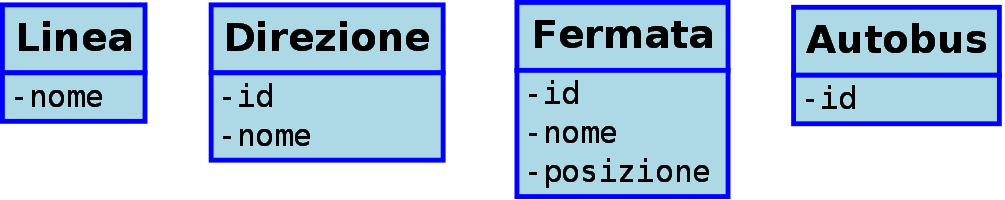
\includegraphics[width=12cm]{contents/images/classi_concettuali}
\end{center}
\caption{Classi concettuali}
\label{fig:classes}
\end{figure}

\newpage
Per ogni classe sono stati definiti anche i corrispettivi attributi d'interesse.

Nel caso della Linea, l'unico dettaglio di cui tenere traccia è il nome, che identifica univocamente la linea nell'insieme globale. Per quanto riguarda la direzione, essa è costituita da un nome di riferimento (usato solo per la consultazione) ed un ID, che ne permette la catalogazione.
Nel caso di Fermata, si può notare l'attributo nome, l'ID e la posizione ove la fermata è collocata, gestita attraverso una coordinata.
Per l'elemento Autobus, l'unico attributo di rilevanza è un ID, il quela permette di identificare un autobus in un vasto insieme di trasporti.

A questo punto si prosegue attraverso la concezione delle relazioni e la creazione delle associazioni tra classi.
Seguendo sempre il caso d'uso descritto in precedenza, una linea contiene un elenco di direzioni, mentre ogni direzione appartiene ad una e una sola linea. Viene quindi creata l'associazione ``Costituita da'' tra Linea e Direzione con molteplicità 1 a N.
Proseguendo, si può notare come a sua volta ogni direzione sia composta da un cospicuo numero di fermate, mentre una fermata può essere un punto di scambio tra più direzioni. Dunque l'associazione ``Composta da'' tra Direzione e Fermata avrà molteplicità N a N.
Concludendo con l'ultima classe, un autobus è associato ad'una direzione univoca e, durante il suo tragitto, si ferma in ogni fermata definita dalla direzione. In una direzione transitano più autobus e, allo stesso modo, in una fermata possono fermare più autobus. Le relazioni tra Autobus e Direzione e Autobus e Fermata saranno definite rispettivamente dall'associazione ``Appartiene'' di molteplicità N a 1 e dall'associazione `Collocato su'' di molteplicità N a 1.
\newpage
Avendo quindi specificato tutte le associazioni essenziali, il diagramma del modello di dominio assume questa forma:

\vspace{1cm}
\begin{figure}[htbp]
\begin{center}
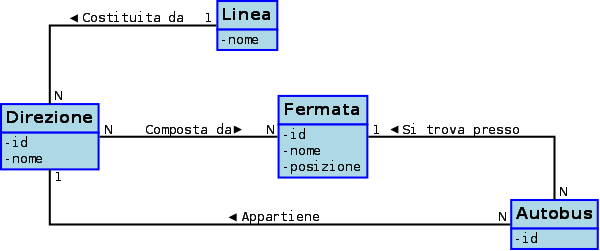
\includegraphics[width=12cm]{contents/images/modelloDominio}
\end{center}
\caption{Classi concettuali}
\label{fig:domain_model}
\end{figure}
\vspace{1cm}

La rappresentazione finale del modello di dominio di questo caso di studio è un diagramma molto semplice e snello, racchiudendo solamente i dettagli essenziali per la progettazione del servizio descritto in questo elaborato.
Come già spiegato in precedenza, il suo scopo non è descrivere in maniera esaustiva il comportamento di un servizio di trasporti urbani, ma si limita a definirne una concezione semplificata e, allo stesso tempo, sufficientemente completa per poter progettare un servizio efficiente.

Nel capitolo seguente si farà riferimento a questo modello di dominio per la definizione del {\itshape diagramma delle classi di progetto}, il quale si assumerà il compito di adattare la visione del modello ad un punto di vista software.
% section il_modello_della_rete_trasporti_pubblici (end)

\newpage

\chapter{Progettazione}\label{cha:progettazione}
In questo capitolo si definiscono le specifiche di progettazione del servizio di visualizzazione dei trasporti pubblici, iniziando con un'introduzione al diagramma delle classi di progetto e l'adattamento del diagramma del modello di dominio concepito nel capitolo precedente ad un punto di vista software.

%%%
%%%possibile introduzione ai frameworks
%%%


\section{Diagramma delle Classi di Progetto} % (fold)
\label{sec:diagramma_delle_classi_di_progetto}

Nel capitolo precedente è stato definito il diagramma del modello di dominio, che rappresenta da un punto di vista grafico le classi concettuali presenti nella realtà di interesse di questa tesi. Esso quindi non rappresenta una modellazione tecnica da poter utilizzare in fase di progettazione, ma si limita a rappresentare in maniera semplice ed essenziale le proprietà e i concetti fondamentali dell'ambiente in studio.
Vi è bisogno dunque di compiere un'ulteriore passo in avanti verso un punto di vista di sviluppo applicativo, rimodellando le classi concettuali del modello di dominio in classi e oggetti software.

Per fare questo, viene utilizzato il diagramma delle classi di progetto, o DCD, il quale scopo è rappresentare in modo dettagliato le classi software, variabili e relazioni così da permettere uno sviluppo efficiente e garantisce una bassa presenza di reiterazioni in fase di implementazione.
% section diagramma_delle_classi_di_progetto (end)

\section{Struttura del DCD} % (fold)
\label{sec:struttura_del_dcd}

Il diagramma delle classi sfoggia una struttura per molti aspetti simile al diagramma del modello di dominio. Essendo una forma avanzata del modello di dominio questo aspetto risulta ovvio, ma dovendosi avvicinare ad una visione orientata puramente allo sviluppo software vi è il bisogno di definire ulteriori dettagli indispensabili nella fase di implementazione.

Seguirà ora una breve descrizione di come gli elementi del modello di dominio siano adattati sotto nuove forme nel diagramma delle classi di progetto.

\subsection{Classificatore} % (fold)
\label{sub:classificatore}

Per quanto riguarda le classi concettuali del modello di dominio, nel diagramma delle classi esse vengono rappresentate attraverso {\itshape classificatori}: un classificatore è un elemento di modello che descrive caratteristiche comportamentali e strutturali. Nel diagramma delle classi i classificatori possono identificare classi regolari o interfacce.

Ogni classificatore dispone inoltre di uno o più attributi o metodi, i quali permettono la conoscenza e l'interazione tra altri classificcatori presenti nel diagramma delle classi.
% subsection classificatore (end)

\subsection{Attributi} % (fold)
\label{sub:attributi_dcd}
Gli attributi di un classificatore sono mostrati in due modi. Essi possono essere elencati all'interno del classificatore, proprio come accade nel modello di dominio, rappresentando così dei contenuti informativi del classificatore.

Nel caso un classificatore abbia un attributo che faccia riferimento ad un'altro classificatore, viene utilizzato l'attributo tramite linea di associazione. Come nel diagramma del modello di dominio, le linee di associazione dispongono di una molteplicità, mentre il verso di percorrenza non è più bidirezionale, ma è orientato verso il classificatore a cui l'origine dell'associazione fa riferimento. Se un oggetto software contiene una collezione di attributi la molteplicità dell'associazione sarà dunque N, od 1 se il riferimento è singolo.
% subsection attributi (end)

\subsection{Operazioni} % (fold)
\label{sub:operazioni}
All'interno del classificatore risiede inoltre un'altra sezione adibita alle {\itshape operazioni}. Nel linguaggio UML, un'operazione è una dichiarazione costituita da nome, parametri e un tipo di valore di ritorno. Inoltre un'operazione può possedere un numero di vincoli che deve soddisfare per essere eseguita.

L'operazione tuttavia non è un metodo, in quanto l'operazione non definisce un'implementazione. Per quella fase si utilizzano per l'appunto i metodi, i quali implementano le operazioni descritte nel diagramma delle classi.
% subsection operazioni (end)

% section struttura_del_dcd (end)

\section{DCD: servizio di visualizzazione dei trasporti} % (fold)
\label{sec:dcd_servizio_di_visualizzazione_dei_trasporti}

Avendo dunque introdotto i concetti e le proprietà del diagramma delle classi di progetto, il prossimo passo è dunque rimodellare il modello di dominio definito nel capitolo precedente in un DCD di elevata fedeltà.

Prendendo dunque come riferimento il modello di dominio, il diagramma delle classi dispone di quattro classificatori principali:\\

{\itshape Linea}

{\itshape Direzione}

{\itshape Fermata}

{\itshape Autobus}\\

Concependo come classi regolari questi quattro oggetti, si prosegue assegnando ad ognuno gli attributi di riferimento e le dipendenze, giungendo ad un diagramma illustrato nella prossima pagina:
\newpage
\vspace{1cm}
\begin{figure}[htbp]
\begin{center}
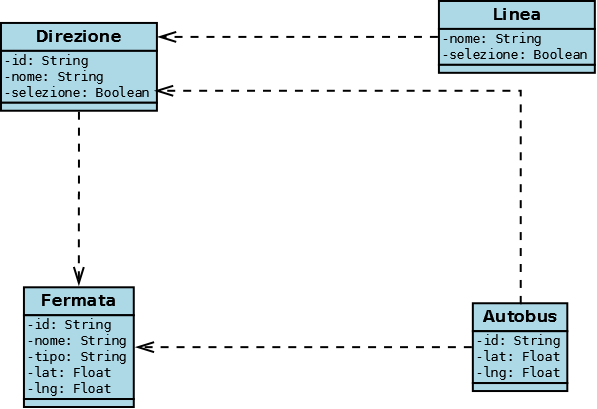
\includegraphics[width=10cm]{contents/images/dcd1}
\end{center}
\caption{Primo diagramma delle classi}
\label{fig:dcd}
\end{figure}
\vspace{1cm}
La classe Linea dispone di un attributo ``nome'' di tipo stringa, ed esso, come nel modello di dominio, assume un ruolo di identificatore nella collezione di oggetti linea che si vuole monitorare.
a Direzione è costituita da un attributo ``id'' e ``nome'', l'id sarà presente anche nelle classi successive, ed è quello che identificherà univocamente le istanze degli oggetti, assegnando invece al nome un contenuto puramente informativo, data la sua eccessiva lunghezza.
Nelle classi Fermata e Autobus sono presenti gli attributi ``latitudine'' e ``longitudine'', i quali definiscono la posizione univoca dell'oggetto nello spazio. Ciò permette la locazione di questi elementi durante la fase di posizionamento sulla mappa di visualizzazione.
Si può notare che le classi Direzione e Linea contiene un attributo ``selezione'', il quale sarà di utilità durante l'implementazione e lo sviluppo, in quanto permette di conoscere le linee e direzioni di preferenza dell'utente.
Infine è stato aggiunto l'attributo ``tipo'' nella classe Fermata, che permette di distinguere una fermata capolinea di partenza, capolinea di arrivo o semplice fermata d'intermezzo.

Per quanto riguarda le dipendenze, la classe Linea ne specifica una verso Direzione, in quanto ogni linea è costituita dalle sue direzioni. Per lo stesso motivo la classe Direzione dispone di una dipendenza verso Fermata. Concludendo con la classe Autobus, esso deve essere assegnato ad una direzione e inoltre deve collocarsi su una fermata, perciò avrà due dipendenze verso le rispettive classi.

Questa prima iterazione del diagramma delle classi di progetto non è però soddisfacente ai fini di sviluppo di un'applicazione web lato client, e deve dunque essere migliorato attraverso l'aggiunta di ulteriori classi che si occupino della gestione delle richieste, il prelievo dei dati, la manipolazione e la visualizzazione di questi ultimi attraverso un'interfaccia.

Possiamo dunque introdurre una classe {\itshape Applicazione}, che sarà la basedia del progetto. Questa classe si occupa di gestire tutte le altre classi e mantenerne i riferimenti.
L'applicazione, per quanto classe {\itshape madre} dell'intero sistema, non deve assurmersi altre responsabilità, come la gestione dei dati e delle richieste degli utenti, in modo da non caricare troppo il suo margine di compiti.

E' opportuno quindi definire una classe {\itshape Controller}. Il compito dell'entità Controller è la cattura e gestione delle richieste che l'utente pone al sito web. Inoltre si occupa della richiesta al server dei dati di interesse all'utente e della loro manipolazione, in modo che siano pronti per una corretta visualizzazione.

Proprio per quest'ultimo aspetto vi è il bisogno di creare una classe {\itshape Vista}, la quale fa riferimento alle classi di dati gestite dal sistema e si occupa della loro visualizzazione ad ogni nuova richiesta e, quindi, cambiamento del set di dati da dover visualizzare.
\newpage
Al seguito di queste nuove scelte progettuali, il nuovo diagramma delle classi assume la forma seguente:

\vspace{1cm}
\begin{figure}[htbp]
\begin{center}
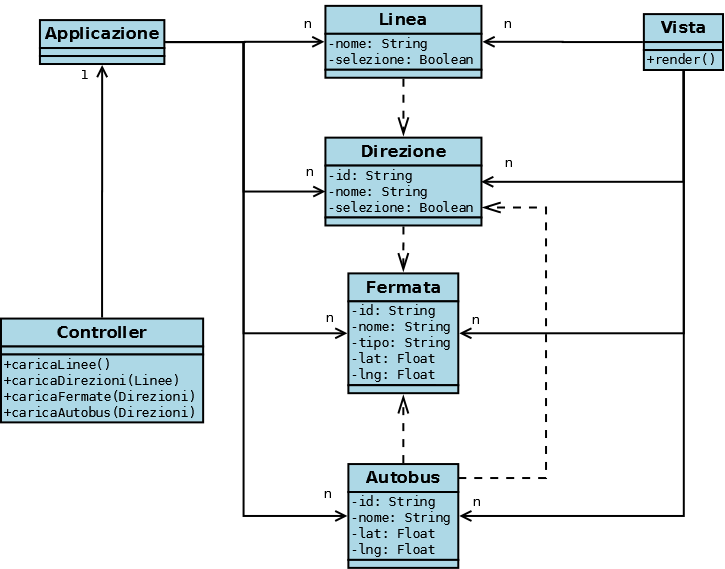
\includegraphics[width=13cm]{contents/images/dcd2}
\end{center}
\caption{Secondo diagramma delle classi}
\label{fig:placeholder}
\end{figure}
\vspace{1cm}

La classe Applicazione, dovendo mantenere dei riferimenti verso le altre classi, dispone di attributi per associazione verso tutte le altre classi definite nel diagramma. Le associazioni verso le classi Linea, Direzione, Fermata e Autobus saranno 1 a N, essendo quest'ultime collezioni di dati di interesse.

La classe Controller dipone di un riferimento verso l'Applicazione, potendo così attingere alle classi di dati e poterle manipolare. Essa dispone dei metodi CaricaLinee(), CaricaDirezioni(linee), CaricaFermate(direzioni) e CaricaAutobus(direzioni), i quali inoltrano una richiesta al server per ottenere i dati di interesse da immagazzinare in modo temporaneo nel client.

\newpage
La classe Vista sarà dotata di riferimenti verso le classi di dati Linea, Direzione, Fermata e Autobus, ed è costituita da un metodo Render(). Questo metodo permette la visualizzazione dei dati prelevati dal server ed immagazinati nel client, dove ognuno disporrà di uno stile di visualizzazione adatto.\\

Attraverso quest'ultima iterazione del diagramma delle classi, si è definito un sistema esaustivo per la creazione di una web application, nei capitoli successivi si descriveranno le scelte progettuali dei framework per lo sviluppo dello struttura lato client e le scelte per la realizzazione dell'interfaccia grafica.

\newpage
% section dcd_servizio_di_visualizzazione_dei_trasporti (end)

\chapter{Frameworks}\label{cha:frameworks}
Dopo aver definito il diagramma delle classi di progetto nel capitolo precedente, si prosegue ora alle scelte di sviluppo per la creazione della struttura di un servizio di consultazione delle linee dei trasporti urbani.

Per quanto riguarda la scelta del linguaggio di programmazione, l'ovvia scelta è ricaduta sul JavaScript, attualmente il linguaggio standard {\itshape de facto} per la realizzazzione di siti e applicazioni web.

JavaScript è un linguaggio di scripting orientato agli oggetti, la cui caratteristica principale è quella di essere un linguaggio interpretato: il codice non viene compilato, ma interpretato (in JavaScript lato client, ogni browser in circolazione ormai dispone di un interprete appropriato).
JavaScript è un linguaggio debolmente tipizzato, in quanto le variabili non devono essere definite da un tipo, ma questo verrà definito ogni volta che verrà assegnato un valore alla variabile. JavaScript è un linguaggio totalmente orientato agli oggetti, ogni variabile ha una struttra array associativa, e permette di definire più proprietà all'interno di una singola variabile.

Un'aspetto fondamentale ai fini di questa tesi è il comportamento di JavaScript lato client: in questo caso il codice viene eseguito direttamente sul client e non sul server. Il vantaggio di questo approccio è che, anche con la presenza di script particolarmente complessi, il server non viene sovraccaricato a causa delle richieste dei clients. Questo linguaggio pone anche alcuni svantaggi: ad esempio, ogni informazione che presuppone un accesso a dati memorizzati in un database remoto deve essere rimandata ad un linguaggio che effettui esplicitamente la transazione, per poi restituire i risultati ad una o più variabili JavaScript; operazioni del genere richiedono il caricamento della pagina stessa, il che comporta ad una cattiva esperienza utente durante la navigazione web. Fortunatamente, con l'avvento della tecnica AJAX questi limiti sono stati superati.\\

Specificato il linguaggio utilizzato per lo sviluppo, vi è bisogno di implementare la struttura definita attraverso il diagramma delle classi di progetto. Facendo riferimento inoltre ai requisiti architetturali specificati nel capitolo \ref{chapter:architettura}, si è preferito fare utilizzo di un framework che permetta uno sviluppo attinente ai paradigmi dell'architettura e facilitare lo sviluppo grazie ad un ambiente con una struttura base già definita.
Allo stato attuale, i framework principali e più famosi per lo sviluppo di applicazioni web sono tre: {\itshape Ember.js}, {\itshape Spine.js} e {\itshape Backbone.js}. Come è possibile notare dal suffisso, le tre piattaforme si basano su JavaScript, e tutti e tre soddisfano requisiti architetturali come MVC e REST.

In ordine di scegliere il framework migliore per lo sviluppo dell'applicazione obiettivo di questa tesi sono stati studiati gli aspetti generici di ogni framework, in modo da valutarne vantaggi e svantaggi mettendoli a confronto.\\

Segue dunque una breve descrizione dei sopracitati framework, in cui verranno specificate le proprietà, i vantaggi e gli svantaggi dello sviluppo su ognuna di queste tre piattaforme.

\newpage

\section{Ember.js} % (fold)
\label{sec:ember_js}

Ember è un framework JavaScript con una struttura fortemente orientata sul pattern MVC. Come gli altri framework offre quindi una struttura di Modelli, Viste e Controlli.

Ember specifica quindi, insieme a molti altri, i moduli per Model, View e Controller, che risultano essere il cuore pulsante della piattaforma.
Oltre a questo, Ember fornisce un sistema per una facile creazione e manipolazione di template, i quali sono di grande aiuto per la visualizzazione di molteplici dati che sono affetti da cambiamenti nel tempo.

Una qualsiasi applicazione web viene definita innanzitutto dai suoi dati. Ember offre una struttura ben congeniata per il salvataggio e la manipolazione dei dati attraverso il modulo Model. Un Model, oltre a contenere dei dati, offre una struttura all'interno di essi per definire ulteriori dati od operazioni sui modelli. Ogni oggetto Model può contenere una o più proprietà, ossia attributi, che specificano informazioni e funzioni che l'oggetto può offrire.

I dati dunque devono essere visualizzati in modo che l'utente possa consultarli ed interagirci. Per far ciò Ember introduce il modulo View, il quale predispone dei metodi di visualizzazione secondo delle direttive imposte dallo sviluppatore facendo uso di un template. Anche se Ember supporta un discreto set di template diversi, quello che Ember usa di default è Handlebars. Handlebars è un famoso linguaggio di templating semantico, il quale immerge nel normale HTML delle semplici espressioni, le quali hanno il compito di visualizzare i dati che gli vengono passati come riferimento in maniera dinamica.

Tornando ai modelli, un singolo modello può contenere un solo dato del tipo definito. Per creare una collezione di modelli dello stesso tipo si fa uso del Controller. In Ember questi moduli vengono chiamati ArrayController, e dal loro nome si intuisce che oltre al semplice contenimento di più dati, offrono anche un set di funzioni definite dallo sviluppatore per manipolare i dati stessi, come prelievo, modifica e salvataggio.
\newpage
Ciò che distingue maggiormente Ember dagli altri framework per lo sviluppo di applicazioni web sono tre caratteristiche particolari:

\begin{itemize}
    \item Bindings
    \item Proprietà computate
    \item Templates ad aggiornamento automatico
\end{itemize}

\subsubsection{Bindings} % (fold)
\label{ssub:bindings}
I bindings, o collegamenti, permettono di mantenere una o più proprietà di oggetti differenti in sincronia. In questo modo una proprietà potrà fare riferimento ad una proprietà di un'oggetto differente e, in caso di una modifica di uno delle due, la modifica verrà propagata anche all'oggetto collegato, evitando dunque il problema di dover modificare più volte attributi presenti in diversi modelli.
% subsubsection bindings (end)

\subsubsection{Proprietà computate} % (fold)
\label{ssub:propriet_computate}
Le proprietà computate permettono di trattare una funzione come una proprietà, specificando nella dichiarazione della proprietà il comportamento della funzione. Il vantaggio è che le proprietà computate funzionano in sinergia coi bindings, e permettono dunque di creare risultati con strutture sia semplici che complesse.
% subsubsection propriet_computate (end)

\subsubsection{Templates ad aggiornamento automatico} % (fold)
\label{ssub:templates_ad_aggiornamento_automatico}
L'aspetto forse più importante di Ember risiede nei templates ad aggiornamento automatico: facendo uso di Handlebars, è possibile immergere in una pagina HTML un riferimento ad uno o più proprietà di un'oggetto di Ember, le quali verranno visualizzate a seconda del valore contenuto in esse. La particolarità è che i template non visualizzano solamente la proprietà, ma mantengono un binding su di essa, in modo che in qualsiasi momento questa cambi, il template modificherà dinamicamente la visualizzazione aggiornandola al nuovo valore.
% subsubsection templates_ad_aggiornamento_automatico (end)

% section ember_js (end)

\section{Spine.js} % (fold)
\label{sec:spine_js}
Spine è il secondo framework su cui si pone l'attenzione in questo studio delle migliori piattaforme per lo sviluppo di WebApp.

Come Ember, Spine offre un'architettura basata sul pattern MVC, potendo servire anche qui moduli per la definizione di dati, visualizzazione, estrazione, manipolazione e salvataggio. Al contrario di Ember, per la visualizzazione Spine non fornisce un sistema di templating già incluso nel framework. Il cavallo di battaglia di Spine è la sua semplicità, questo framework infatti è composto solo da moduli essenziali, e lascia tutto il resto alla libertà di scelta dello sviluppatore.

\subsubsection{Model} % (fold)
\label{ssub:spine_model}

Al fine di definire dei dati da manipolare in un ambiente client, Spine fornisce il modulo Model, nel quale i dati caricati dal server vengono immagazzinati e risultano pronti per la modifica. I modelli sono il cuore di Spine, ed oltre ad immagazzinare dati possono, come Ember, contenere delle funzioni logiche associate alle informazioni contenute negli oggetti.
A differenza di Ember (e Backbone, come si vedrà in seguito), i modelli di Spine non garantiscono una definizione delle proprietà in maniera dinamica (ergo l'aggiunta di proprietà in un'istanza anche dopo che il modello è stato definito), ma necessitano di essere configurate durante la dichiarazione del modello.
Un'altra caratteristica unica di Spine è l'assenza di collezioni: questa piattaforma non fornisce dei moduli per la gestione di molteplici istanze di un modello. In ogni Model di spine vengono forniti i metodi save() e load(), i quali, se richiamati, sincronizzano il modulo con il server, salvando o caricando l'istanza in remoto.
% subsubsection model (end)
\newpage
\subsubsection{View} % (fold)
\label{ssub:spine_view}

Per la visualizzazione dei dati, Spine usa un modulo Vista unico tra i framework presi in studio: nella terminologia di Spine, le Viste sono semplici frammenti di codice HTML che compongono l'interfaccia dell'applicazione. Questa piattaforma non dispone di widget per la realizzazione di interfacce e non detta alcuna struttura base per la struttura delle viste. Tutto è lasciato a discrezione dello sviluppatore.

Per una visualizzazione dinamica e strutturata dei dati su una pagina web vi è bisogno quindi di immergere il codice in un testo HTML, separando i due aspetti tramite opportuni tag per la distinzione del linguaggio HTML da quello applicativo.
In altre parole, si può affermare che in Spine non esiste una View vera e propria.
% subsubsection view (end)

\subsubsection{Controller} % (fold)
\label{ssub:spine_controller}

Riguardo la gestione dei dati, Spine fornisce un modulo di controllo, il Controller per l'appunto. A differenza di Ember, in Spine non costituisce una collezione di modelli, ma assume il semplice ruolo di delegare delle funzioni a seconda della ricezione di eventi definiti nella sua dichiarazione. Alla sua dichiarazione, vi è il bisogno di associare un elemento del DOM al Controller. Dopodiché sarà possibile definire un set di eventi generati da elementi situati all'interno dell'elemento specificato, associati ad una o più funzioni, anch'esse dichiarate all'interno della struttura del controller.
% subsubsection controller (end)

% section spine_js (end)
\newpage

\section{Backbone.js} % (fold)
\label{sec:backbone_js}

L'ultimo framework posto sotto analisi è Backbone. Come le altre due piattaforme descritte in precedenza, Backbone fornisce una struttura avanzata per lo sviluppo di applicazioni web fornendo modelli per la realizzazione di strutture dati, delle collezioni per una gestione contemporanea di più modelli e delle viste provviste di una struttura di event handling.

Al contrario di Ember e Spine, Backbone non dichiara mai di possedere una struttura basata sul pattern MVC. Infatti Backbone non fornisce un modulo per la creazione di controller ma, come si potrà vedere, gli aspetti tralasciati da questa mancanza vengono recuperati in qualche modo da altri moduli.

Backbone brilla grazie alla sua struttura semplice e pratica, offrendo un framework leggero e snello per chi ha bisogno di sviluppare un'applicazione web di modeste proporzioni ma mantenendo un'architettura di discreta complessità così da permettere la realizzazione di siti web più avanzati.

\subsubsection{Model} % (fold)
\label{ssub:backbone_model}

Anche in Backbone, come negli altri framework, viene fornita una struttura per la rappresentazione di dati tramite modelli. Come si può ormai intuire, questo modulo offre caratteristiche assai simili alla controparte dei suoi avversari, permettendo di definire dei dati attraverso un'elenco di proprietà che possono a loro volta rappresentare semplici contenuti informativi o funzioni logiche definite per la fornitura e manipolazione dei dati presenti all'interno del modello.
Una particolarità dei modelli di Backbone è la loro natura spontanea nel generare eventi di cambio di stato. Al momento della creazione di un modello, esso viene automaticamente collegato ad un oggetto evento, che si occuperà di notificare chiunque sia in ascolto non appena avvenga una modifica nel Model.
% subsubsection model (end)

\subsubsection{Collection} % (fold)
\label{ssub:backbone_collection}
Diversamente da Ember e Spine, Backbone fornisce in modo esplicito un modulo per la collezione di uno o più oggetti di uno stesso modello.
Collection dunque rappresenta un insieme ordinato di modelli. Al momento della sua definizione, vi è il bisogno di specificare una proprietà model che permetterà alla collezione di riconoscere i tipi di dato di cui deve tener traccia.
Attraverso le collezioni, Backbone fornirce metodi semplici e diretti per operare su gruppi di dati, facendo uso dell'unica libreria richiesta obbligatoriamente al setup di questo framework: {\itshape Underscore.js}. In breve, Underscore è una libreria che offre numerose funzioni per lo scorrimento, filtraggio, modifica e ricerca su gruppi di dati.
Una Collection inoltre può contenere una o più funzioni, proprio come accade nei modelli, in modo da poter definire metodi per la gestione e l'estrapolazione di uno o più dati presenti nella collezione.
Un'altra peculiarità delle collezioni di Backbone è la caratteristica di ``ereditare'' gli eventi generati dal modello che la collezione integra. In questo modo, ad esempio, non appena un'oggetto della collezione notifica un cambio di stato, l'intera collezione notificherà a sua volta questo tipo di evento, cosicché eventuali ascoltatori sulla collezione potranno accorgersi del cambiamento ed operare di conseguenza.
% subsubsection collection (end)

\subsubsection{View} % (fold)
\label{ssub:backbone_view}
Il modulo View è ciò che permette a Backbone la visualizzazioni dei dati rappresentati nei modelli. Da come sono strutturati, essi non definiscono niente della struttura HTML o del CSS al posto dello sviluppatore, ma fanno utilizzo di una qualsiasi libreria JavaScript per il  templating. L'idea generale di Backbone è quella di organizzare un'interfaccia tramite una o più viste, anche annidate tra loro, le quali possono far riferimento sia ad un singolo modello che ad una collezione di essi. Ogni vista può quindi essere aggiornata autonomamente non appena il modulo o la collezione di riferimento attua un cambio di stato, così da non aver bisogno di riscrivere l'intera pagina.
E' dunque possibile definire delle funzioni associate a determinati eventi del modulo di riferimento, in modo tale che la vista possa sempre monitorare le continue modifiche del modello e possa agire su di esse in modo coerente. Si può notare come questa peculiarità avvicina molto la vista al concetto di Controller, e in effetti la View è il modulo che per più aspetti simula lo strato controllore.
% subsubsection view (end)

% section backbone_js (end)
\newpage


\section{Caratteristiche comuni e valutazioni finali} % (fold)
\label{sec:caratteristiche_comuni_e_valutazioni_finali}

Oltre ai principali tre moduli che definiscono la struttura MVC di Ember, Spine e Backbone, tutti e tre i framework implementano inoltre altre caratteristiche comuni per la gestione delle rotte in un sito web. Una di particolare importanza è il Router.

\subsubsection{Router} % (fold)
\label{ssub:router}
Il modulo Router è la risorsa essenziale al fine di creare un'applicazione web dinamica e composta da una struttura di sezioni tale che l'applicazione possa rispondere in maniera adeguata a seconda della sezione in cui si trova.

L'url di un sito web rappresenta l'indirizzo in cui possono essere recuperate determinate risorse. Ogni volta che viene inserito un nuovo url, il browser invia una richiesta a quell'indirizzo, effettuando il caricamento di una nuova pagina se ciò che gli viene passato è un indirizzo legale.
Una convenzione degli url tuttavia si basa sull'utilizzo del carattere ``\#'' per evitare l'aggiornamento della pagina. Definendo meglio questo aspetto, si può dire che durante l'inserimento di un url, tutto ciò che viene descritto al seguito del carattere \# viene accettato dal browser, ma non comporta un nuovo caricamento del sito web.

Su quest'aspetto si basa il modulo Router: esso rimane in ascolto sui cambiamenti dell'url sul server a cui fa riferimento e cattura ogni rotta descritta immediatamente dopo il tag \#. Successivamente ne verifica la corrispondenza con delle rotte definite all'interno della sua struttura e, se viene trovato un confronto, invoca una chiamata alla funzione associata a quella rotta.

In questo modo è possibile definire infiniti comportamenti che l'applicazione web può eseguire a seconda di quale sezione l'utente stia facendo accesso, in modo da poter caricare i dati opportuni o visualizzare delle informazioni specifiche.
% subsubsection router (end)


\subsection{Valutazioni} % (fold)
\label{sub:valutazioni}

Si conclude dunque la descrizione dei tre principali framework candidabili allo sviluppo di un'applicazione web discutendo sui loro aspetti di forza e le loro debolezze, mettendo a confronto le principali caratteristiche delle tre piattaforme.

Riguardo ai modelli, vi sono poche differenze in termini di struttura di questi moduli nei tre framework, in quanto tutti e tre offrono un sistema di proprietà e definizione di funzioni all'interno del Model.
La vera distinzione giunge attraverso l'aspetto di gestione di multiple istanze dei modelli. Con Ember, è possibile dichiarare un controller che venga adibito al monitoraggio di un gruppo di modelli attraverso una struttura array. Attraverso Backbone tutto ciò è reso ancora più chiaro grazie all'uso dei moduli Collection, che rappresentano in modo pratico il concetto di collezione e offrono inoltre un sistema di notifica annidata degli eventi dei modelli. Sfortunatamente in Spine non è presente un modulo concreto per la memorizzazione di più oggetti, e l'unico modo per ovviare a questo problema è un salvataggio dei dati su un server.

Riguardo ai metodi per la visualizzazione dei dati, i più veloci ed intuitivi risultano quelli di Ember. Attraverso un processo di auto-aggiornamento implementato insieme ai template, Ember permette allo programmatore di definire solo dove il dato venga visualizzato, dopodiché egli non avrà più bisogno di preoccuparsene. Similmente, ma in maniera meno diretta, le viste di Backbone permettono di aggiungere dei template aggiornabili tramite funzioni {\itshape event driven}, ed è possibile inoltre poter annidare più viste in modo da iterare la visualizzazione anche su collezioni di dati. Il tutto risulta in un metodo di visualizzazione più esplicito e meno ``magico'' come quello della controparte Ember, permettendo al programmatore di agire in modo assoluto sui meccanismi di visualizzazione. Per quanto riguarda Spine, anche in questo aspetto il framework non fornisce un metodo accattivante quanto quello delle sue controparti. La scrittura di codice applicativo all'interno di codice HTML risulta dispersiva e poco leggibile, e si preferisce dunque staccare queste due componenti.

Per lo strato di controllo i framework Spine e Ember offrono per alcuni aspetti un sistema simile tra loro: il controller definisce degli eventi a cui deve tener traccia, ed ogni volta che uno degli eventi definiti si presenta, il controller eseguirà la funzione associata a quell'evento. In Backbone invece non è presente un Controller ``tangibile'', ma le sue metodologie sono implementate a grandi linee nel modulo View.
% subsection valutazioni (end)

\subsubsection{La scelta} % (fold)
\label{ssub:la_scelta}
Dovendo sviluppare un'applicazione web che gestisca un sistema informativo dei trasporti urbani, vi è un forte bisogno di una gestione di molteplici collezioni dei vari oggetti, i metodi di gestione devono essere i più diretti possibile per consentire uno sviluppo fluido. Da questo punto di vista Backbone sembra la scelta migliore grazie alla sua definizione chiara di collezioni.
Per quanto riguarda lo strato di visualizzazione il framework più appetibile risulta Ember, tuttavia Backbone fornisce una struttura chiara e concisa la quale, in sinergia con le collezioni, consente una visualizzazione altamente personalizzabile e manipolabile sia degli insiemi che dei singoli dati.

Un'altro elemento che ha influito sulla scelta di Backbone è il suo grado di semplicità: l'applicazione che si vuole sviluppare deve risultare semplice ed essenziale, tuttavia ha il bisogno di gestire e visualizzare anche un gran numero di informazioni contemporaneamente.
Da queste necessità, si è preferito Backbone alla complessa struttura di Ember e a quella fin troppo semplice di Spine.

Dunque d'ora in poi, durante la realizzazione del servizio, si farà riferimento agli elementi specifici del framework Backbone.js.
% subsubsection la_scelta (end)

% section caratteristiche_comuni_e_valutazioni_finali (end)

\newpage

\chapter{Realizzazione}\label{cha:realizzazione}
\section{Programmazione modulare} % (fold)
\label{sec:programmazione_modulare}

Una volta appreso JavaScript si nota come questo linguaggio di programmazione abbia oltre ai suoi pregi anche alcuni punti deboli.
Nativamente JavaScript non fornisce alcun sistema di modularizzazione, si cerca quindi di rendere modulare il codice attraverso le seguenti tecniche: 
\begin{itemize}
    \item Il codice viene definito attraverso funzioni le quali sono richiamate immediatamente dopo la loro dichiarazione.
    \item I riferimenti dalle dipendenze sono fatti attraverso variabili globali le quali vengono caricate in ambiente HTML tramite appositi tag script.
    \item Le dipendenze sono dichiarate in modo debole: il programmatore ha bisogno di sapere l'ordine esatto delle dipendenze. Ad esempio, per definire una classe Direzione che si riferisca ad una Fermata, la classe Fermata deve essere definita prima di Direzione
    \item Il caricamento degli script lato client può diventare in certi casi molto lento e deve essere ottimizzato
\end{itemize}

Tutto ciò può diventare difficoltoso in caso di progetti complessi, in modo particolare quando gli script cominciano ad avere molte dipendenze, le quali tendono a sovrapporsi e nidificarsi. Inoltre la definizione manuale dei tag script non è scalabile, e non offre la possibilità di caricare gli script su richiesta.

\subsubsection{Common.js} % (fold)
\label{ssub:common_js}
Per ovviare a questo problema, Common.js, d'ora in poi CJS, definisce un formato di modularità che si interfaccia col linguaggio JavaScript odierno, ma non è necessariamente costretto dalle limitazioni degli ambienti JavaScript presenti nei browser. Per assicurare una compatibilità tra l'ambiente di sviluppo e il browser, CJS utilizza un metodo di traduzione dei moduli in un formato interpretabile dl browser. Il formato di modularità di CJS permette la presenza di un solo modulo per file, perciò vi è il bisogno di un ``formato di trasposizione'' per accorpare più moduli in un unico file, cercando di ottimizzare il codice al massimo.

In questo modo CJS si è potuta concentrare su come ovviare al problema delle dipendenze circolari, oltre che a creare dei riferimenti alle dipendenze. Tuttavia, non è riuscita a risolvere tutti i problemi, come il caricamento asincrono dei dati. Inoltre le misure di compatibilità imposte dai browser pongono un ulteriore problema per gli sviluppatori; effettuare debugging su un singolo file, mentre lo sviluppo avviene su più file, risulta difficoltoso.
% subsubsection common_js (end)
\subsubsection{AMD} % (fold)
\label{ssub:amd}
AMD (Asynchronous Module Definition) si occupa di ovviare anche agli ultimi problemi di CJS. L'obiettivo del formato AMD è quello di fornire una soluzione al problema della modularità in JavaScript, per poter essere usata immediatamente dagli sviluppatori.

AMD è un formato per la definizione di moduli, dove sia moduli che dipendenze possono essere caricate in modo asincrono. AMD si basa sulla pratica di CJS per definire le dipendenze ed i riferimenti ma al contrario di common.js permette anche la definizione di più moduli in un singolo file, se necessario.
% subsubsection amd (end)
\newpage
\subsubsection{Brunch} % (fold)
\label{ssub:brunch_io}
Al fine di utilizzare tali formati, si è scelto di adottare un application assembler quale {\itshape Brunch}.

Brunch, basandosi sui formati AMD e Common.js, offre una struttura modulare, offrendo metodi di riferimento ed esportazione dei moduli. I moduli sono definiti all'interno di un file JavaScript, ed organizzati in cartelle in maniera opportuna. Brunch rimane in osservazione per eventuali modifiche dei file, e per ognuna di esse, compila tutti gli script ed eventuali template in moduli Common.js.

L'applicazione generata con Brunch è definita da un esiguo numero di file statici, i quali possono essere poi trasferiti in qualsiasi altro ambiente. Brunch offre anche un'opzione di {\itshape minify}, che permette una ``compilazione'' del codice in maniera ristretta, per garantire un caricamento più rapido lato client.

Brunch è inoltre completamente agnostico a qualsiasi tipo di framework, libreria, linguaggio di programmazione e templating. Permette dunque una buona libera di scelta lasciando però allo sviluppatore la comodità di scrivere codice senza doversi preoccupare di definire moduli adeguati ai formati AMD e CJS.

Al fine di introdurre lo sviluppatore immediatamente alla programmazione minimizzando la fase di setup, Brunch definisce inoltre un set di ``scheletri''. Gli scheletri sono delle impostazioni personalizzabili che forniscono un buon punto di inizio per lo sviluppo di nuove applicazioni. Ogni Scheletro definisce un determinato framework, uno o più linguaggi e librerie.
% subsubsection brunch_io (end)
% section programmazione_modulare (end)
\newpage

\section{Sviluppo} % (fold)
\label{sec:sviluppo}
Avendo definito tutti gli strumenti di sviluppo, si prosegue ora alla creazione del progetto.

Il funzionamento base di questo servizio si basa su questo elenco di passaggi:

\begin{enumerate}
    \item l'utente accede al sito web per la consultazione dei trasporti pubblici
    \item il client richiede al server le linee autobus che sono monitorate dal servizio
    \item il client carica le informazioni delle linee e le visualizza all'utente
    \item l'utente seleziona una o più linee di sua preferenza, e procede con la visualizzazione delle direzioni
    \item il client richiede al server le direzioni di cui ha bisogno, specificando le linee selezionate
    \item il client carica le informazioni delle direzioni e le visualizza all'utente
    \item l'utente seleziona una o più direzioni che vuole consultare, e procede alla loro visualizzazione sulla mappa
    \item il client richiede al server le fermate delle direzioni di cui ha bisogno, specificando le direzioni
    \item il client carica le informazioni delle fermate e le visualizza all'utente su una mappa
    \item il client richiede al server gli autobus in circolazione sulle direzioni di cui ha bisogno, specificando le direzioni
    \item il client carica le informazioni degli autobus e li visualizza all'utente su una mappa
\end{enumerate}
\newpage

I requisiti progettuali imposti all'inizio della progettazione richiedono che l'esperienza utente non sia limitata ad uno scorrimento sequenziale di questi punti dal numero 1 all'11, ma possa anche iniziare da punti successivi al primo, attraverso l'inserimento di un url che passi parametri correttamente interpretabili dal client.

Dopo aver specificato il caso d'uso relativo al servizio web, si proceda con la definizione delle base del progetto: il modulo Application.

\subsection{Application} % (fold)
\label{sub:application}

Il modulo Application è definito come il ``padre'' di tutti gli altri moduli presenti in questo progetto.
La sua struttura è molto semplice: non dispone di proprietà, in quanto questo modulo non deve contenere alcun tipo di contenuto informativo, ma solo richiedere e mantenere i riferimenti degli altri moduli del progetto, così da poter servire in caso di bisogno gli altri moduli.

Application definisce un solo metodo, \code{initialize()}, all'interno del quale l'Application carica tutti i moduli, quali collezioni, viste e router, con l'apposito metodo fornito da Brunch. Una volta caricati tutti i moduli richiesti, l'applicazione procede alla loro inizializzazione passando come parametri eventuali proprietà necessarie. 

Application sarà quindi l'unico modulo importato nella pagina HTML di riferimento dell'applicazione attraverso il tag \code{<script>} e, attraverso la chiamata al metodo \code{initialize()} si occuperà di caricare tutti gli altri moduli.
% subsection application (end)

\subsection{Modelli del servizio} % (fold)
\label{sub:modelli_del_servizio}

Avendo dunque definito la struttura base della nostra applicazione, si proceda con la definizione e creazione del cuore del servizio: i modelli.

Seguendo le specifiche del diagramma delle classi di progetto definite nel capitolo \ref{cha:progettazione}, vi è il bisogno di definire quattro modelli: Linea, Direzione, Fermata e Autobus.

Come esempio dimostrativo, verrà mostrata la sintassi di definizione del modello Direzione:

\begin{lstlisting}
var Model = require('core/Model');

var Direction = Model.extend({
    defaults: {
        id: "",
        name: "",
        checked: false,
        },
    changeChecked: function() {
        this.checked = !this.checked;
    }
});

module.exports = Direction;
\end{lstlisting}

Innanzitutto vieni importato il modulo Model, il quale mette a disposizione tutte le funzionalità base del modulo Model di Backbone.
Segue dunque la definizione del modello Direction estendendo con le opportune proprietà/metodi la classe base.
L'hash \code{defaults} permette di specificare gli attributi di base che ogni modello deve contenere. Quando viene creata un'istanza del modello, se uno qualsiasi degli attributi contenuti all'interno di \code{defaults} non viene specificato, esso sarà impostato al suo valore di default.
Per il modello Direzione, vengono specificati le proprietà definite come attributi nel diagramma delle classi di progetto realizzato nel capitolo \ref{cha:progettazione}. La proprietà \code{checked} farà riferimento alla casella di selezione specifica all'istanza del proprio modello, e verrà invocato il metodo \code{changeChecked()} ogniqualvolta la casella sarà selezionata o deselezionata.

Una volta definito il modello si definisce la sua esportazione che ne garantisce un riferimento per gli altri moduli.

Una volta terminata la costruzione della struttura portante dell'applicazione, si può proseguire alla specifica del fulcro dell'applicazione web: il modulo Router.
\newpage

\subsection{Router} % (fold)
\label{sub:router}

Il Router è il modulo fondamentale per la realizzazione di un'applicazione web moderna, consentendo, tramite il suo sistema di rotte, una navigazione dei contenuti del sito web senza aver bisogno di ricaricare la pagina.
Attraverso una strutturazione in sezioni ben definita nelle rotte, il router può comprendere ciò che l'utente sta richiedendo al servizio, ed è capace di richiamare apposite funzioni che si occupano di richiedere al server i dati di cui si ha bisogno e salvarli quindi sul client.

Inoltre attraverso il router è possibile lasciare una traccia nella cronologia di navigazione, consentendo in questo modo all'utente di poter scorrere attraverso i passaggi effettuati all'interno del sito web.

La struttura principale del router è definita nel codice seguente. Per evitare un eccessiva lunghezza di codice sono stati omessi i contenuti delle funzioni.

\begin{lstlisting}
var Router = require('core/Router');

var application = require('Application');
ApplicationRouter = Router.extend({
    routes: {
        '': 'home'
        'lines': 'loadLines'
        'lines/:lines' : 'loadLines',

        'lines/:lines/directions' : 'loadDirections',
        'lines/:lines/directions/:directions' : 'loadDirections',

        'lines/:lines/directions/:directions/stations' : 'loadMap'
    },

    <all functions are listed below>
});

module.exports = ApplicationRouter;
\end{lstlisting}
\newpage

Come in ogni definizione di nuovi moduli, ApplicationRouter importa il modulo Router che garantisce le funzionalità base messe a disposizione da Backbone. 
All'interno di ApplicationRouter viene definita la proprietà \code{route}, il quale conserva al suo interno i riferimenti tra le rotte che il router deve riscontrare e le funzioni che verranno invocate nel caso il riscontro associato ad esse sia positivo.

La struttura della rotta è stato uno degli aspetti su cui si è posta maggiore attenzione, in quanto uno degli obiettivi prefissati per questo progetto è consentire una navigazione interattiva grazie ad una manipolazione dinamica dell'indirizzo.

\subsubsection{modellazione dinamica dell'url} % (fold)
\label{ssub:modellazione_dinamica_dell_url}

% subsubsection modellazione_dinamica_dell_url (end)

Una delle idee su cui poggiano le fondamenta della costruzione di questa applicazione web si basa sulla possibilità di poter costruire un url in modo dinamico, inserendo in esso i vari parametri che il fruitore del servizio ha selezionato tramite l'interfaccia utente.
Ogniqualvolta l'utente seleziona una linea e/o direzione di preferenza, la composizione dell'indirizzo cambia in tempo reale, in modo tale che alla premuta del tasto di conferma, esso sia già pronto per una corretta lettura da parte del Router.

L'aggiornamento dell'url avviene attraverso l'utilizzo del metodo nativo \code{navigate} del modulo Router. \code{navigate} permette la navigazione verso un indirizzo che deve essere passato come parametro al metodo. Inoltre ad ogni chiamata di \code{navigate} l'indirizzo a cui si vuole navigare viene salvato nella cronologia, questo comportamento può essere evitato attraverso il passaggio di appositi parametri.

In questo progetto l'aggiornamento delle rotte viene effettuato dalle collezioni \ref{sec:collezioni}. Esse conoscendo gli elementi selezionati  possono costruire la rotta corrispondente nella maniera opportuna.
% subsection subsection_name (end)
\newpage

La struttura dell'indirizzo web concepita per questa applicazione è la seguente, essa viene esposta nella sua completezza, ma durante la navigazione del servizio l'url verrà ``composto'' un passo alla volta:

\begin{lstlisting}
   lines/:lines/directions/:directions/stations
\end{lstlisting}

l'indirizzo è suddiviso nella sezione linee, la sezione direzioni ed infine la sezione stazioni. In Backbone, un elemento nella rotta avente i  due punti di prefisso rappresenta un parametro. \code{:lines} e \code{:directions} contengono quindi le linee e le direzioni che l'utente ha scelto di consultare, le quali sono definite attraverso il loro codice identificativo

Lo scopo di questi parametri è duplice: ad esempio, se la sezione dei parametri delle è l'ultima porzione dell'indirizzo (come \code{lines/:lines}), vuol dire che si sta richiedendo l'elenco di tutte le linee, e che quelle presenti nel parametro sono già selezionate. Il router quindi richiederà al server tutti gli oggetti linea e li salverà nella collezione, dopodiché provvederà ad impostare le proprietà \code{checked} degli oggetti linea che corrispondono a quelli elencati nel parametro.
Se invece al parametro sussegue un'ulteriore porzione di url (come \code{lines/:lines/directions...}), il router comprenderà che si stanno richiedendo degli oggetti Direzione, e per specificare al server di quali direzioni si ha bisogno invierà nella richiesta anche il parametro delle linee.

La composizione dell'indirizzo in sezioni è inoltre utile ai fini dell'utente: dopo aver selezionato per la prima volta le linee e direzioni che si vogliono consultare, l'url rappresenta un link simbolico a quel set di preferenze. Quindi l'utente potrà salvare l'indirizzo e riutilizzarlo per accedere immediatamente alla visualizzazione degli autobus in circolazione, senza dover ripetere il processo di selezione ancora e ancora.

\vspace{1cm}

Tornando al Router, si può notare come le rotte siano definite in tre gruppi distinti: ogni gruppo rappresenta un tipo di sezione che il Router deve saper interpretare ed elaborare. Per ogni gruppo viene chiamata rispettivamente la funzione \code{loadLines}, \code{loadDirections} e \code{loadMap}, dove ognuno è adibito al prelievo delle rispettive risorse. Il nome dell'ultimo metodo non è chiaro: la funzione non si occupa del caricamento della mappa dal server, ma racchiude in se il prelievo degli oggetti fermata e autobus, i quali verranno poi posizionati sulla mappa già disponibile sulla pagina web.

Descrivendo le funzioni di prelievo dei dati si continua a far riferimento al caso delle linee: la funzione \code{loadLines} si occupa di richiedere al server tutte le linee monitorate dal servizio.

Per prima cosa dunque richiede all'Application la collezione linee, e su questa invoca il metodo \code{fetch}, il quale invia una richiesta AJAX al server di riferimento (per ulteriori dettagli consultare la sezione \ref{sec:collezioni}). Se i dati vengono caricati correttamente si imposteranno le proprietà \code{checked} delle istanze linea riscontrate nel parametro.

\subsection{Collezioni} % (fold)
\label{sub:collezioni}

% subsection collezioni (end)
Descritta la definizione dei modelli e conclusa la trattazione del Router, fondamentale per la piena comprensione di questa sezione, si procede alla costruzioni delle entità capaci di gestire molteplici istanze dei modelli: le Collections.

Focalizzandosi sempre sulla direzione, la struttura base per la definizione di una collection è la seguente:

\begin{lstlisting}
var Collection = require('core/Collection');
var Direction = require('models/Direction');

var Directions = Collection.extend({
    
    model: Direction,
    
    url: '/directions',
    
    initialize: function() {
        this.on("change", this.setSelectedOnUrl);
    },
    parseSelected : function() {
        ...
    },    
    setSelectedOnUrl: function() {
        this.setUrl(false)
    },
   setUrl: function(trigger, tail, head) {
        ...
        router.navigate(this.prefix + this.url, {trigger: trigger})
        }   
    },
    goToStation: function() {
        router.navigate(url.join('/'), {trigger: true, replace:true})
    }
});

module.exports = Directions;
\end{lstlisting}

Come nella dichiarazione dei modelli, la collezione crea un riferimento alla struttura base Collection e al modello opportuno.

La collezione oltre a dover conoscere il modello di riferimento dovrà essere inizializzata con un \code{url}. Tale proprietà indicherà alla collezione la rotta su cui richiedere le informazioni per istanziare/modificare i propri modelli.

La funzione \code{fetch} è forse la più importante tra quelle offerte dal modulo Collection, in quanto in essa si basa la struttura di richieste dei dati al server. Per facilitare la comprensione, precedentemente si era affermato che il Router si facesse carico delle richieste dati al server e per poi caricarli nel client. Quest'affermazione è inesatta, dato che in realtà Backbone delega questo compito direttamente alla collezione. Attraverso \code{fetch}, la collezione invia una richiesta AJAX al server aspettandosi una risposta in formato JSON, la quale contiene una collezione di dati di struttura identica a quella del modello cui la collezione fa riferimento.
La funzione \code{fetch} inoltre incorpora le {\itshape callback} \code{success} ed \code{error}, le quali verranno invocate rispettivamente nel caso di una ricezione corretta dei dati o dalla presenza di un errore nella risposta.

Le collezioni di Backbone dispongono anche di una struttura di {\itshape event handling}: è possibile impostare un {\itshape event handler} tramite il comando \code{this.on(event, callback)}. Il primo parametro che gli verrà passato sarà il tipo di evento da ascoltare, in questo caso il cambiamento di un oggetto nella collezione, mentre come secondo parametro verrà passata la funzione adibita alla gestione di quell'evento.

Per quanto riguarda gli altri metodi definiti all'interno della Collection, essi sono adibiti alla costruzione del frammento url che verrà passato al Router, così da poter aggiornare l'indirizzo in base alle preferenze espresse dall'utente.

Il principio di funzionamento è il seguente: attraverso l'{\itshape event handler} definito al momento della creazione, la collezione rimane in ascolto di eventuali cambiamenti. Non appena un modello viene modificato (ciò vuol dire che il suo attributo checked è cambiato), il compito della collezione è di aggiornare la stringa che rappresenta il parametro delle direzioni selezionate. Per fare ciò, viene invocato il metodo \code{setSelectedOnUrl}, il quale delega il compito di aggiornamento dell'indirizzo al metodo \code{setUrl(trigger, tail, head)}.

 \code{setUrl(trigger, tail, head)} richiede tre parametri: il primo rappresenta il parametro \code{option} che deve essere passato alla funzione navigate di Router, mentre \code{tail} e \code{head} corrispondono alle porzioni di indirizzo che dovranno essere poste prima e dopo alla sezione che si vuole modificare.
 All'interno di \code{setUrl} viene richiamata la funzione \code{parseSelected()}, la quale ha il compito di fornire la stringa contenente gli oggetti che sono stati selezionati: per fare ciò la funzione attua un filtraggio degli elementi con attributo \code{selected} affermativo, e prosegue generando una stringa contenente la concatenazione degli identificatori delle direzioni.

 Una volta ricevuto il parametro, la funzione \code{setUrl} compone il frammento di indirizzo concatenando il prefisso, il parametro e la suffisso, e prosegue all'invocazione del metodo \code{navigate} di Router.

 Il metodo \code{goToStation} è una versione semplificata del metodo \code{setUrl}, il quale viene invocato alla pressione del tasto di conferma nell'interfaccia. \code{goToStation}

\subsection{Viste} % (fold)
\label{sub:viste}

Attraverso le viste è infine possibile visualizzare all'utente i dati di cui ha bisogno filtrati e modellati attraverso le scelte che ha effettuato durante la navigazione del servizio.
La struttura generale di una Vista di Backbone è la seguente:

\begin{lstlisting}
var View     = require('core/View');
var template = require('templates/DirectionTemplate');

var DirectionView = View.extend({
      
      template: template,

      events: {
      ...
      }

      initialize {
      ...
      }

      render {
      ...
      }
}

module.exports = DirectionView;
\end{lstlisting}


Oltre ad importare le funzioni standard offerte dal modulo View di Backbone, nella definizione di una nuova vista vi è il bisogno di importare un template costruito in precedenza, il quale fornisce alla vista la struttura HTML per la visualizzazione dei dati a cui la vista fa riferimento.
Alla creazione di una vista è possibile passare una o più di opzioni le quali saranno attribuite alla vista tramite \code{this.options}. Esistono inoltre alcuno opzioni speciali che possono essere attribuite direttamente alla Vista, quali \code{model}, \code{collection}, \code{el}, \code{id}, \code{attributes} \code{className} e \code{tagName}. All'interno della View può essere definita la funzione di inizializzazione, la quale sarà chiamata al momento della creazione della vista.

La proprietà \code{el} definisce un elemento del DOM a cui la vista fa riferimento in ogni momento. Tramite questo riferimento, la vista può effettuare una visualizzazione dei dati all'interno del suo elemento \code{el} in qualsiasi momento, non intaccando il resto della struttura HTML. L'elemento \code{el} viene creato dalle proprietà \code{tagName}, \code{className}, \code{id} e \code{attributues}, oppure può essere assegnato ad un'elemento preesistente nel DOM. Nel caso nessuna di queste opzioni venga adottata, \code{el} rappresenterà un \code{<div>} vuoto.
Le proprietà \code{model} e \code{collection} permettono di creare un riferimento tra la vista e l'oggetto (o collezione di oggetti) che si deve visualizzare.

Oltre al ruolo di visualizzatori dati, l'altra natura delle Viste di Backbone è quella di rappresentare un Controller. La Vista gestisce un set di eventi specificati all'interno della proprietà \code{events}, i quali sono assegnati a delle funzioni che verranno richiamate ogniqualvolta un determinato evento occorre.
In questo modo è possibile garantire una visualizzazione dinamica dei dati attribuendo la funzione \code{render()} all'evento di cambio di stato generato dall'oggetto cui fa riferimento la View. In questo modo si ottiene una rappresentazione sempre aggiornata dell'elemento, senza avere il bisogno di ulteriori caricamenti della pagina.
Oltre alla gestione degli eventi al fine di visualizzare il dato, l'uso degli eventi può garantire anche una manipolazione dei dati cui la Vista fa riferimento.
Ad esempio, per garantire che gli oggetti linea (o direzione) siano notificati della loro selezione, è stato creato un evento \code{'.click'} della casella di selezione associata all'oggetto della View. Non appena la casella viene selezionata, l'evento viene catturato dalla vista, la quale richiama la funzione \code{changeChecked()} del modello, impostando in modo corretto il valore della sua proprietà.

Tornando alla visualizzazione dei dati, la vista svolge questo compito attraverso l'uso del metodo \code{render()}. Inizialmente questo metodo non svolge nessuna funzione, e deve essere quindi sovrascritto dal programmatore con operazioni cui lui ritiene più opportune.
Generalmente all'interno della funzione \code{render} viene associato il template di riferimento della View al suo elemento del DOM, nel quale il template può essere ridisegnato ogni volta o appeso. E' buona norma in Backbone inserire un \code{return this} alla fine della funzione \code{render} in modo da abilitare chiamate concatenate tra le viste.

Infine le viste possono essere annidate, in modo da consentire una struttura gerarchica all'apparato di visualizzazione. Durante lo sviluppo del progetto è state definita ad esempio la vista \code{DirectionView}, la quale si propone come un singolo elemento dell'elenco di direzioni, rappresentato da \code{DirectionsView}. Quest'ultima, insieme alla vista \code{MapView} è contenuta all'interno di una vista ``madre'' chiamata \code{MainView}, la quale rappresenta l'intero body della pagina e definisce la macro-struttura dell'interfaccia del servizio.
% subsection viste (end)

\subsection{Templating} % (fold)
\label{sub:templating}

Uno dei problemi che bisogna affrontare durante la fase di visualizzazione dei dati sull'interfaccia web è il tipo di metodologia con cui rappresentare le informazioni in modo dinamico. In un applicazione web la struttura funzionale viene sempre gestita attraverso un linguaggio di programmazione quale JavaScript, in cui le risorse vengono gestite e organizzate. Invece per quanto riguarda la sua interfaccia essa si basa, ovviamente, sul linguaggio fondamentale del web, l'HTML.

Dunque per poter essere in grado di rappresentare in modo dinamico le informazioni gestite nell'applicazione web, vi è il bisogno di escogitare un metodo di conversione per essere in grado di ``tradurre'' i dati strutturati in JavaScript in modo tale da poter essere visualizzati tramite HTML.

La soluzione più semplice a questo problema risiede nella possibilità di incorporare JavaScript direttamente all'interno dell'HTML. Per differenziare i due linguaggi in modo che siano interpretati correttamente si utilizzano degli appositi tag che definiscono dove il linguaggio JavaScript inizia e termina all'interno di un documento HTML. Tuttavia questa soluzione risulta poco elegante, in quanto l'utilizzo di due linguaggi differenti in uno stesso documento rende la lettura poco chiara e comprensibile. E' buona norma quindi fare in modo che i due linguaggi siano ben distinti e separati, permettendo solo la comunicazione delle informazioni che si vogliono rappresentare.

I template ricoprono questa funzione, svolgendo un ruolo di ``ponte'' tra la struttura logica e quella rappresentativa. In un template è possibile descrivere una struttura HTML in cui il dato deve essere visualizzato, quest'ultimo viene passato al template come parametro, e viene riconosciuto correttamente grazie all'uso di un preciso tag. Per comunicare i dati ad un template esso può essere richiamato all'interno dell'applicazione similmente ad una chiamata di funzione, in cui i parametri passati rappresentano le informazioni da visualizzare.

I template sono {\itshape logic-less}, ciò vuol dire che la filosofia generale di un template sia quella di contenere meno struttura logica possibile al loro interno. Tutto ciò che deve essere incorporato in un template deve riguardare la semantica, evitando la presenza di cicli o condizioni. Inoltre i template tendono a seguire il principio {\itshape DRY}, che sta per {\itshape Don't Repeat Yourself}. L'idea di base è che ogni informazione deve essere descritta in una struttura rappresentativa una sola volta, cosicché se essa debba essere visualizzata più volte non vi sia bisogno di ridefinire l'informazione ma riapplicare solamente la struttura che la contiene.

\subsubsection{Mustache} % (fold)
\label{ssub:mustache}
Un template molto diffuso che fa uso di questi principi è {\itshape Mustache}.
Una tipica sintassi di Mustache è la seguente: \lstinline!Hello {{name}} {{lastname}}!. Gli elementi contenuti all'interno dei tag {{}} costituiscono il nome dei parametri che vengono passati al template tramite formato JSON, con la tipica forma:
\begin{lstlisting}
    {"name": "Valerio", "lastname": "Lanziani"}
\end{lstlisting}
Quando il template verrà renderizzato, al posto dei nomi dei parametri verranno visualizzati i rispettivi valori. Oltre alla visualizzazione di semplici stringhe, Mustache permette attraverso i tag \lstinline!{{#list}}{{/list}}! il passaggio di collezoni di oggetti, i quali verrano visualizzati in modo sequenziale all'interno dei due tag. Allo stesso modo è possibile passare come parametri dei metodi che dovranno tornare come valore la stringa che si desidera mostrare.

Per quanto Mustache offra in modo sintetico le funzionalità base per una visualizzazione pulita e comprensibile delle informazioni, questo template pecca di fin troppa semplicità.
Non è ad esempio possibile, se si dispongono di strutture dati nidificate, poter estrarre l'informazione desiderata: Mustache richiede sempre e solo un'informazione diretta dal parametro che gli viene passato.
Essendo un template {\itshape logic-less} Mustache non integra quindi semplici funzioni logiche che potrebbero tornare utili durante la visualizzazione di una struttura particolarmente complessa.
% subsubsection mustache (end)

\subsubsection{Handlebars} % (fold)
\label{ssub:handlebars}
Per ovviare a questi problemi si è fatto uso del template {\itshape Handlebars}.
Handlebars applica gli stessi principi {\itshape DRY} e {\itshape logic-less} come Mustache, pur offrendo delle semplici funzioni logico che possono tornare utili in fase di rendering.

Handlebars garantisce una completa compatibilità con il template Mustache, offrendo lo stesso tipo di sintassi descritta in Mustache. E' dunque possibile importare direttamente l'intera struttura creata con Mustache in un template Handlebars, così da poter iniziare subito ad usufruire delle caratteristiche introdotte da questo template.

Nel caso si disponga di una struttura dati nidificata come, ad esempio:
\begin{lstlisting}
    {"fullname": {"name": "Valerio", "lastname": "Lanziani"}}
\end{lstlisting}
Non sarebbe possibile con Mustache la richiesta del valore ``name''. Tramite Handlebars, è possibile invece utilizzare la sintassi \lstinline!{{fullname.name}}! per permettere al template di rappresentare anche informazioni nidificate.

Handlebars fornisce anche la possibilità di definire degli Helpers, ossia delle funzioni a cui è possibile passare dinamicamente uno o più parametri. Attraverso la sintassi \lstinline!{{{link line}}}! è possibile richiamare la funzione link definita nel template nel modo seguente:
\begin{lstlisting}
Handlebars.registerHelper('link', function(line) {
  return new Handlebars.SafeString(
    "<a href='" + line.url + "'>" + line.text + "</a>"
  );
});
\end{lstlisting}
Durante la chiamata dunque \code{link} rappresenta il nome della funzione mentre \code{line} è il parametro che gli viene passato.
% subsubsection handlebars (end)

% subsection templating (end)


% section sviluppo (end)



\chapter{Esempi d'uso e dimostrazioni}\label{cha:dimostrazioni}
In questo capitolo verranno mostrati gli esempi d'uso ed alcune dimostrazioni di come funzioni il servizio sviluppato.\\

Accedendo alla pagina iniziale, il servizio carica tutte le linee monitorate (per motivi di semplicità sono state usate solo quattro linee):
\vspace{1cm}
\begin{figure}[htbp]
\begin{center}
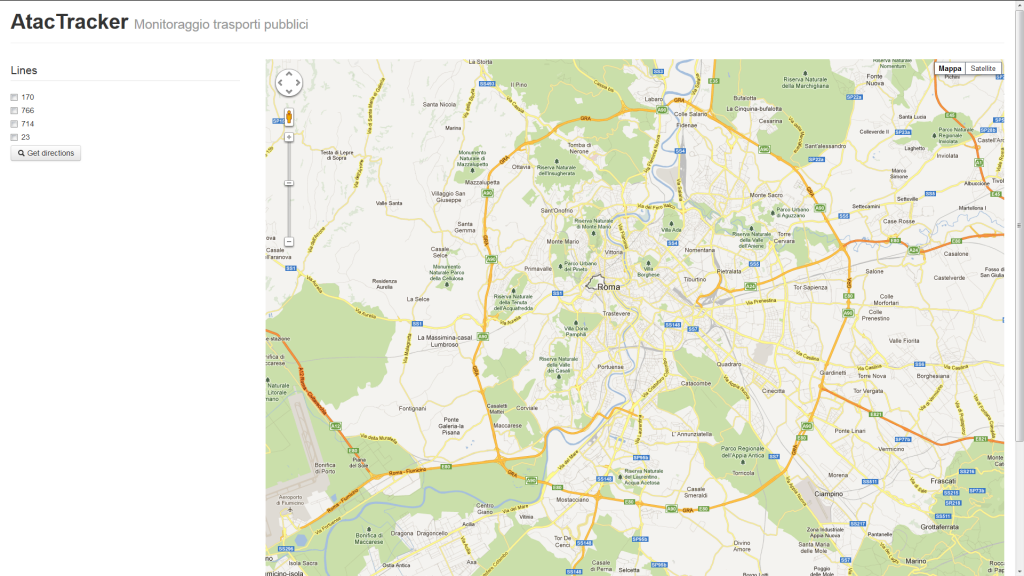
\includegraphics[width=13cm]{contents/images/home}
\end{center}
\caption{Pagina iniziale}
\label{fig:fermata}
\end{figure}

\newpage
Al momento della selezione delle linee scelte, il servizio prosegue richiedendo le direzioni appartenti a quelle linee per poi visualizzare all'utente, come si può constatare nella seguente figura:

\begin{figure}[htbp]
\begin{center}
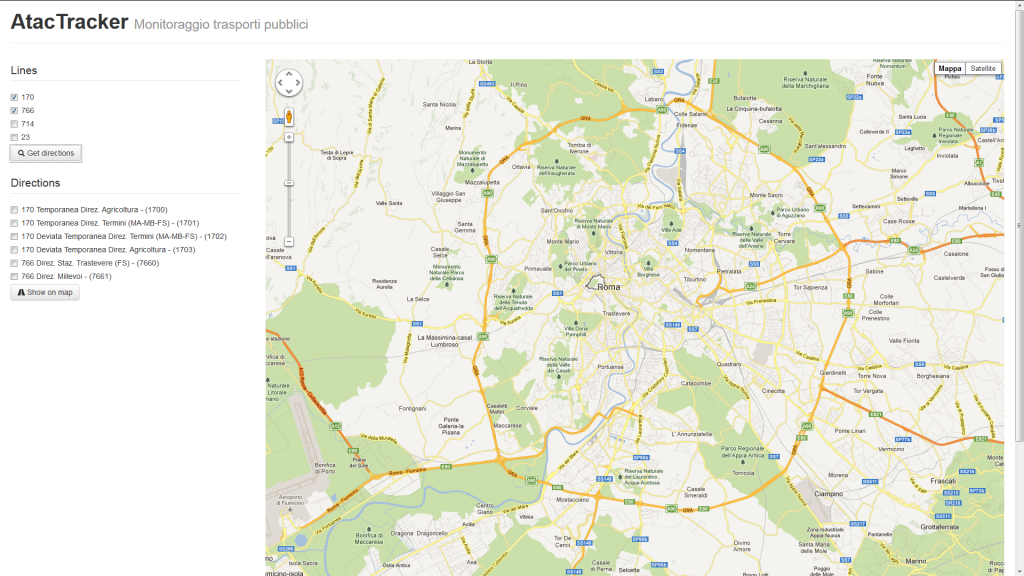
\includegraphics[width=13cm]{contents/images/directions}
\end{center}
\caption{Lista delle direzioni}
\label{fig:fermata}
\end{figure}

E' possibile notare come l'url sia composto dinamicamente in base alle scelte dell'utente, in base ai cambi di scelta che vengono richiesti, l'indirizzo viene assemblato con i giusti parametri:

\begin{figure}[htbp]
\begin{center}
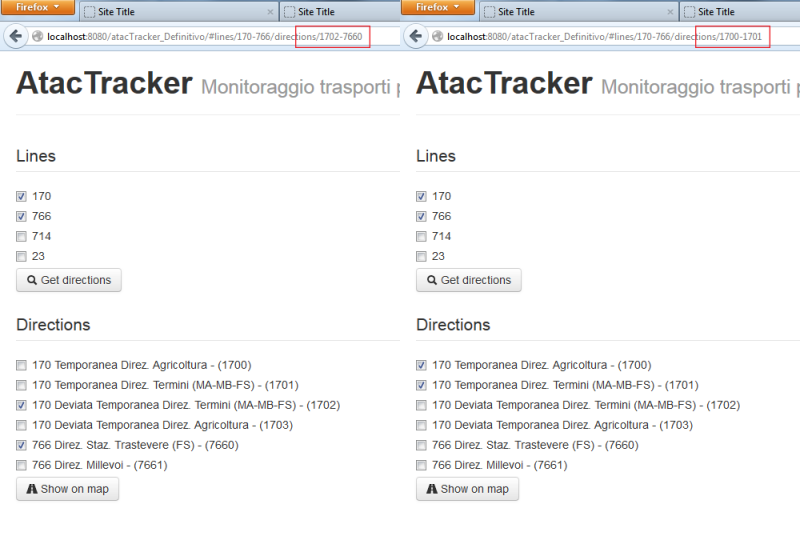
\includegraphics[width=12cm]{contents/images/indirizzo}
\end{center}
\caption{Modifica dinamica dell'url}
\label{fig:fermata}
\end{figure}
\newpage
Una volta selezionate le direzioni preferite e premuto l'apposito pulsante verranno visualizzate tutte le fermate inerenti a quelle direzioni e tutti gli autobus in circolazione presso quei tragitti, distinti tramite l'uso di marcatori di colore e forma differente.

Una semplice legenda aiuta l'utente a poter distinguere una direzione da un'altra:

\begin{figure}[htbp]
\begin{center}
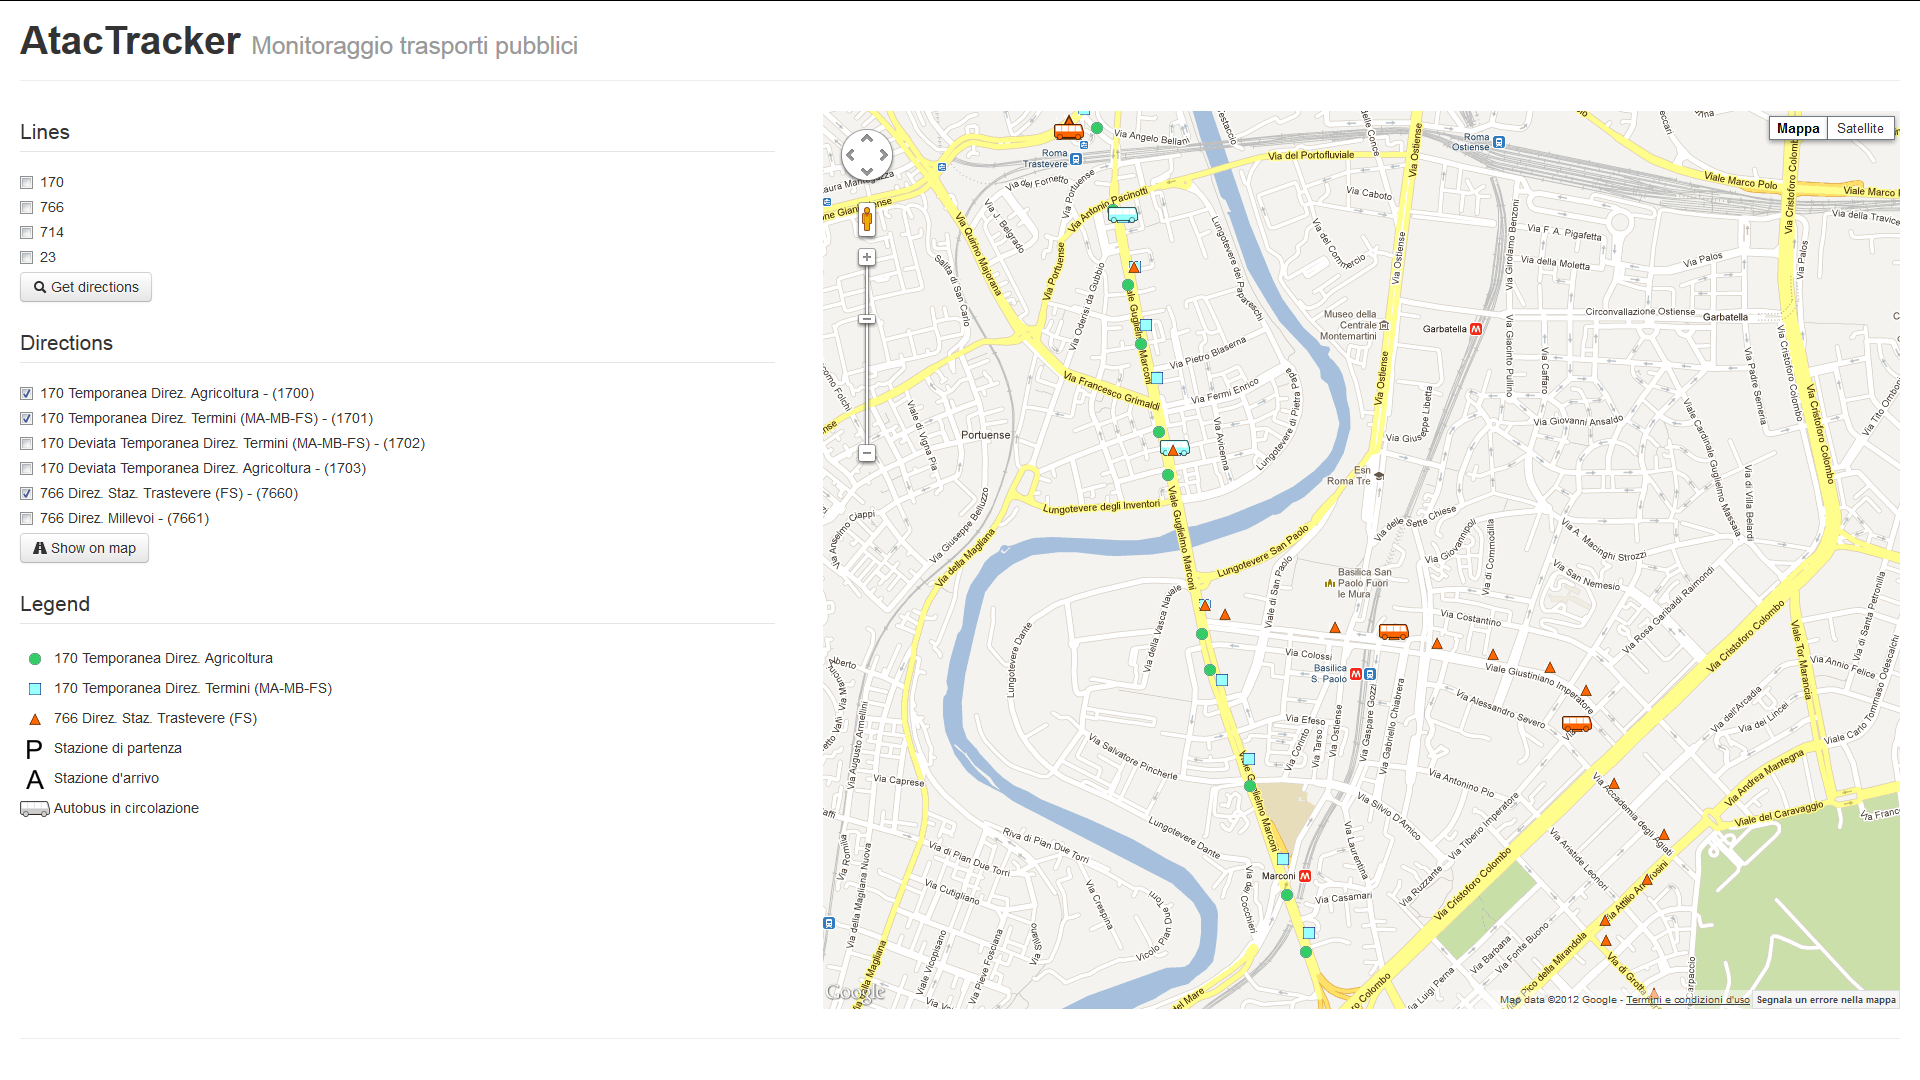
\includegraphics[width=13cm]{contents/images/bus}
\end{center}
\caption{Visualizzazione su mappa}
\label{fig:fermata}
\end{figure}

Col passare del tempo il servizio aggiornerà automaticamente la situazione degli autobus, aggiornando la mappa con le nuove posizioni:

\begin{figure}[htbp]
\begin{center}
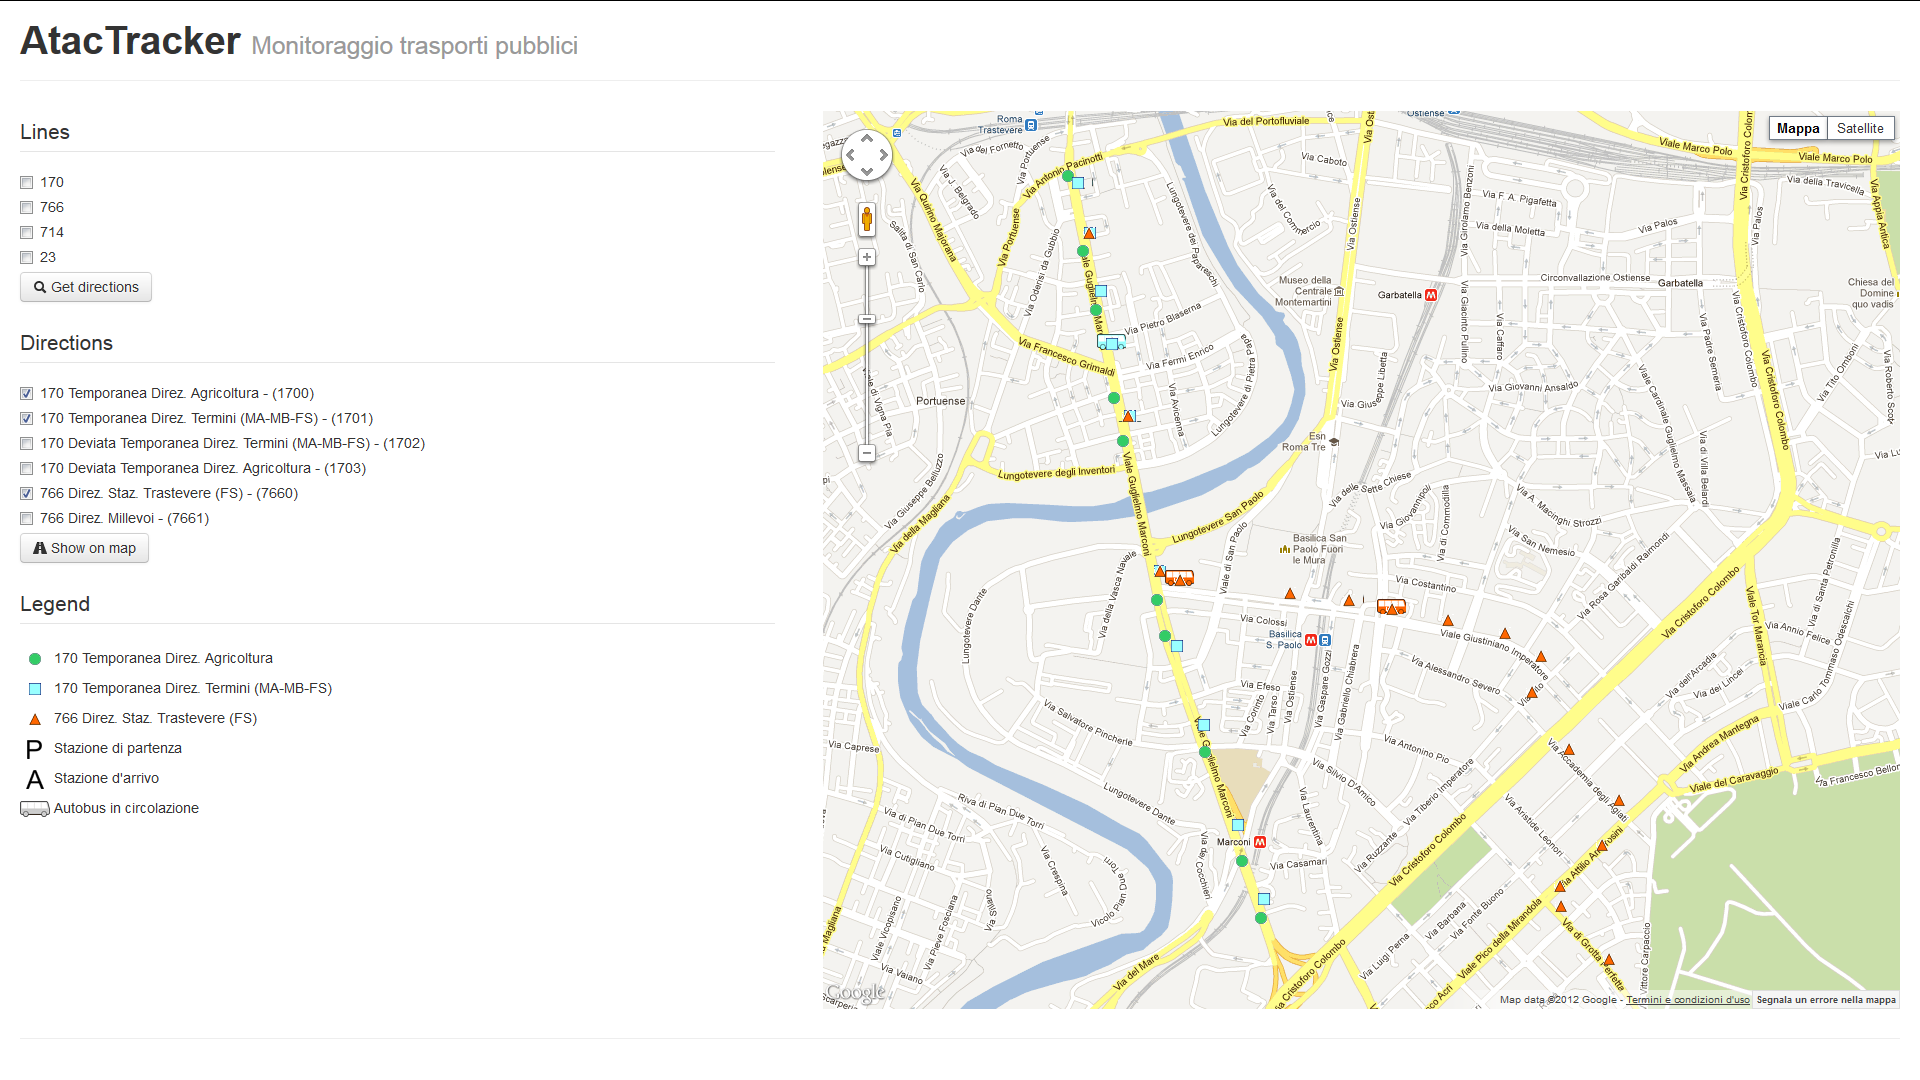
\includegraphics[width=13cm]{contents/images/bus2}
\end{center}
\caption{Visualizzazione dopo un minuto}
\label{fig:fermata}
\end{figure}
\newpage
Concludendo, si mostra come lo sviluppo di un sistema con Responsive Design permetta una corretta visualizzazione su qualunque dispositivo e qualunque risoluzione. Stringendo il browser, infatti, il sito si adatterà ai nuovi parametri di altezza e lunghezza, riposizionaro i vari elementi in modo opportuno:

\begin{figure}[htbp]
\begin{center}
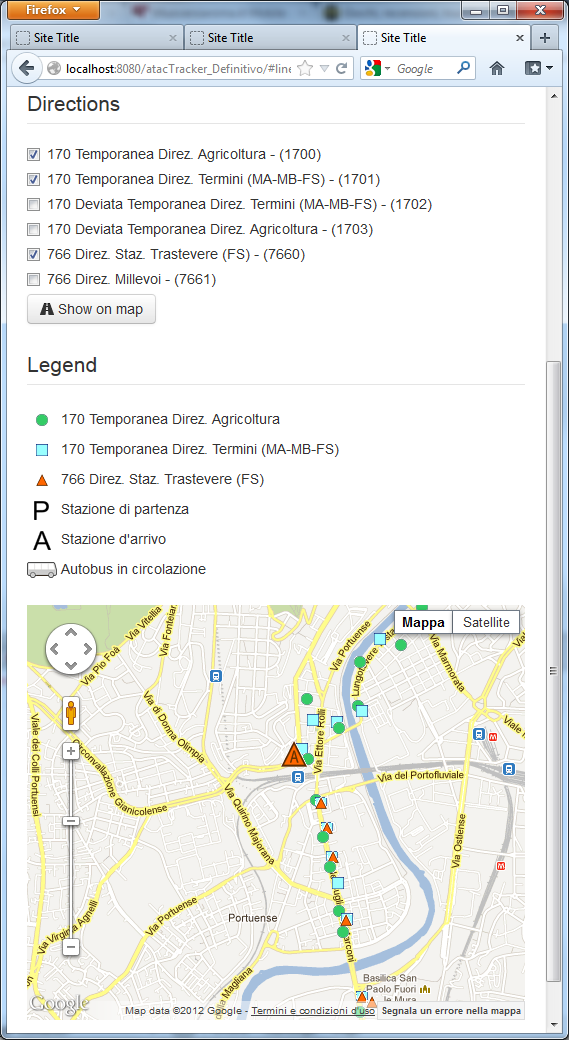
\includegraphics[height=15cm]{contents/images/responsive}
\end{center}
\caption{Visualizzazione con risoluzioni verticali}
\label{fig:fermata}
\end{figure}


\chapter{Conclusioni e sviluppi futuri}\label{cha:conclusioni}
Alla conclusione di questo elaborato può essere affermato di aver risolto il requisito principale dello sviluppo di questo servizio: l'applicazione web visualizza in modo opportuno tutte le direzioni richieste dall'utente, offrendo una corretta rappresentazione delle stazioni lungo una o più linee prescelte.\\

Il servizio soddisfa anche i requisiti di visualizzazione degli autobus in transito lungo la direzione, rendendo noto all'utente a che punto del tragitto essi si trovino. Grazie all'intregazione di una funzione temporizzata, è inoltre possibile ora l'aggiornamento della situazione degli autobus in modo automatico, aspetto completamente assente nel sito web predefinito della rete di trasporti di Roma.\\

Un'altro traguardo raggiunto riguarda la corretta visualizzazione dell'interfaccia web su diverse piattaforme, quali smartphone, tablet e computer: l'interfaccia web si adatta a piccoli schermi assumendo un'impostazione verticali, mentre nel caso di visualizzazione su schermi widescreen essa viene automaticamente impostata ad una rappresentazione orizzontale permettendo di avere sotto controllo tutte le sezioni dell'applicazione web.

\newpage

\subsubsection{Sviluppi futuri} % (fold)
\label{ssub:sviluppi_futuri}

Allo stato attuale l'applicazione permette di mostrare l'ubicazione delle fermate e degli autobus richiesti dall'utente, ma non fornisce la possibilità di notificare la posizione in cui egli si trova. Il servizio potrebbe essere quindi ulteriormente migliorato tramite l'implementazione dei metodi di geolocalizzazione offerti da HTML5, in modo tale da poter suggerire all'utente le stazioni a lui più vicine effettuando un calcolo tra la sua posizione e le coordinate delle fermate appartenenti alle direzioni di preferenza.\\

Un altro aspetto che può essere approfondito riguarda l'implementazione delle WebSockets, sempre offerte da HTML5, per la realizzazione di una comunicazione bidirezionale tra server e client. Al momento l'aggiornamento automatico è permesso tramite una richiesta temporizzata di nuovi dati al server, il quale può comportare un eccessivo numero di richieste che il server deve gestire nel caso l'applicazione dovesse servire un bacino d'utenza molto ampio. Attraverso le WebSockets il client sarebbe in grado di inviare solamente la prima volta le preferenze dell'utente al server, ricevendo successivamente in maniera completamente asincrona dati sempre aggiornati riguardo l'ubicazione degli autobus.
% subsubsection sviluppi_futuri (end)

% chapter conclusioni (end)
% ...other chapters here

%\chapter{Examples}\label{chapter:examples}
%%
This Chapter presents some examples for those of you who are not familiar with the \LaTeX and the packages used in this templates. \\
%
\section{Acronyms}
%
\begin{itemize}
	\item \gls{ABC} 	% Basic usage, this is what you get the first time you use an acronym
	\item \gls{ABC}		% ... and the second time
	\item \glspl{ABC}	% ... and the standard plural
	\item \acrshort{DEF}	% Short version even if used for the first time
	\item \gls{DEF}		% ... the first non-short version
\end{itemize}
%
\section{Citations}
%
\begin{itemize}
	\item \cite{whyinternetjustworks} 	% Simple citation, for more fancy stuff look for the natbib package
	\item \cite{berkeleyclouds,art-and-asl} % Multiple citation
\end{itemize}
%
\clearpage
%
\section{Figures}
%
\begin{center} 					% center whatever is inside
	\begin{figure}[htbc]			% the 'figure' env... htbc = preferences "here,top,bottom,center"
	
\includegraphics[width=0.95 \linewidth]{contents/images/image_test} % width and image location
	\caption{Just a picture}
	\label{label:for:reference}		% you can use this to refer the picture with: \ref{label:for:reference}
	\end{figure}
\end{center}
%
\section{Tables}
%
\begin{center}
 \begin{table}[htbc]				% Table env..
  \begin{tabular}{ l | l }			% Tabular env... GIYF
    \hline
    Column 1 & Column 2 \\
    \hline
    Lorem ipsum dolor sit amet & consectetur adipiscing elit. Curabitur pharetra venenatis odio \\
    Lorem ipsum dolor sit amet & consectetur adipiscing elit. Curabitur pharetra venenatis odio \\
    Lorem ipsum dolor sit amet & consectetur adipiscing elit. Curabitur pharetra venenatis odio \\
    \hline
  \end{tabular}
  \label{table:label:for:reference}		% as with figures, \ref{table:label:for:reference}
  \caption{Just a table}			% Table caption
 \end{table}
\end{center}
%


% Starts roman page numbering
%\newpage
%\setcounter{page}{1}
%\pagenumbering{roman}

% Appendixes
\appendix
\chapter{Appendix A Title}\label{apx:API}
%
Lorem ipsum dolor sit amet, consectetur adipiscing elit. Curabitur pharetra venenatis odio, ac pellentesque nulla blandit at. Maecenas eget massa arcu. Duis tempor justo et sapien ornare pulvinar. Nullam sollicitudin aliquet dui, in fermentum tortor ornare eu. Duis cursus vehicula semper. Donec condimentum felis ut dolor malesuada imperdiet. Nam ullamcorper, tortor vitae mattis cursus, magna nulla interdum diam, sit amet egestas mi turpis nec metus. Ut eu est vitae dolor facilisis viverra. Praesent id erat eu diam semper tincidunt. Curabitur condimentum sem in neque gravida pulvinar. Aliquam vitae neque quis neque vehicula suscipit. Duis at purus felis. Vestibulum id ante ipsum. \\

Donec sit amet dui a arcu condimentum accumsan. Aliquam magna velit, pretium vitae placerat vel, mattis ut sapien. Aliquam porttitor ipsum quis risus ultricies non lacinia lorem laoreet. Integer elementum sollicitudin pulvinar. Donec sed ullamcorper orci. Suspendisse pretium ante ligula, a dapibus leo. Phasellus feugiat mauris vel lacus faucibus non ultricies ipsum placerat. Curabitur pellentesque odio nec eros egestas non pellentesque metus aliquam. Sed enim enim, interdum consequat consectetur sed, faucibus eu quam. Curabitur arcu massa, lacinia eu varius a, tempor id lacus. Praesent ultrices porttitor ligula, vitae consequat erat elementum eu. Aliquam vitae egestas justo. In hac habitasse platea dictumst. Ut interdum accumsan odio, eu commodo nunc laoreet vitae. Praesent purus nibh, tincidunt at viverra ut, bibendum quis lorem. Morbi convallis augue quis velit rhoncus non tristique est commodo. \\

Curabitur in nisi ipsum, id porta mauris. Pellentesque tempus risus nec justo pharetra ac eleifend quam congue. Phasellus eget gravida est. In dapibus imperdiet tristique. Sed quis laoreet nisi. Aliquam erat volutpat. Lorem ipsum dolor sit amet, consectetur adipiscing elit. Proin dignissim blandit nunc, et luctus libero vulputate ac. Duis a diam ac mauris aliquam sodales. Proin faucibus vehicula vehicula. Sed faucibus lorem eget orci imperdiet quis faucibus leo volutpat. Vivamus in consectetur arcu. In aliquet euismod elit, a pretium magna eleifend adipiscing. Etiam semper dui sit amet ante cursus commodo eleifend diam mollis.

%\chapter{Appendix B Title}%
Lorem ipsum dolor sit amet, consectetur adipiscing elit. Curabitur pharetra venenatis odio, ac pellentesque nulla blandit at. Maecenas eget massa arcu. Duis tempor justo et sapien ornare pulvinar. Nullam sollicitudin aliquet dui, in fermentum tortor ornare eu. Duis cursus vehicula semper. Donec condimentum felis ut dolor malesuada imperdiet. Nam ullamcorper, tortor vitae mattis cursus, magna nulla interdum diam, sit amet egestas mi turpis nec metus. Ut eu est vitae dolor facilisis viverra. Praesent id erat eu diam semper tincidunt. Curabitur condimentum sem in neque gravida pulvinar. Aliquam vitae neque quis neque vehicula suscipit. Duis at purus felis. Vestibulum id ante ipsum. \\

Donec sit amet dui a arcu condimentum accumsan. Aliquam magna velit, pretium vitae placerat vel, mattis ut sapien. Aliquam porttitor ipsum quis risus ultricies non lacinia lorem laoreet. Integer elementum sollicitudin pulvinar. Donec sed ullamcorper orci. Suspendisse pretium ante ligula, a dapibus leo. Phasellus feugiat mauris vel lacus faucibus non ultricies ipsum placerat. Curabitur pellentesque odio nec eros egestas non pellentesque metus aliquam. Sed enim enim, interdum consequat consectetur sed, faucibus eu quam. Curabitur arcu massa, lacinia eu varius a, tempor id lacus. Praesent ultrices porttitor ligula, vitae consequat erat elementum eu. Aliquam vitae egestas justo. In hac habitasse platea dictumst. Ut interdum accumsan odio, eu commodo nunc laoreet vitae. Praesent purus nibh, tincidunt at viverra ut, bibendum quis lorem. Morbi convallis augue quis velit rhoncus non tristique est commodo. \\

Curabitur in nisi ipsum, id porta mauris. Pellentesque tempus risus nec justo pharetra ac eleifend quam congue. Phasellus eget gravida est. In dapibus imperdiet tristique. Sed quis laoreet nisi. Aliquam erat volutpat. Lorem ipsum dolor sit amet, consectetur adipiscing elit. Proin dignissim blandit nunc, et luctus libero vulputate ac. Duis a diam ac mauris aliquam sodales. Proin faucibus vehicula vehicula. Sed faucibus lorem eget orci imperdiet quis faucibus leo volutpat. Vivamus in consectetur arcu. In aliquet euismod elit, a pretium magna eleifend adipiscing. Etiam semper dui sit amet ante cursus commodo eleifend diam mollis.


% Acronyms and Glossary
%\newpage
%\glsaddall
%\renewcommand{\glsgroupskip}{}
%\printglossary[type=\acronymtype,style=long,title=Table of Acronyms]

%\newpage
%\printglossary[style=altlist,title=Glossary]

% Bibliography
\cleardoublepage
\phantomsection
\addcontentsline{toc}{chapter}{Bibliography}
% Uncomment the following line if you want all of the bib entries to be displayed
\nocite{*}
\bibliographystyle{\mybibstyle}
\footnotesize{
 \bibliography{contents/other/references_url.bib}
%}

\end{document} 
